% Bao cao nhom: Song song hoa mo phong N-body bang OpenMP va CUDA
% Bien dich (XeLaTeX):  latexmk -xelatex bao_cao.tex   hoac   make report  (o thu muc goc repo)
\documentclass[12pt,a4paper,oneside]{report}
\usepackage[fontsize=13pt]{scrextend}

% ================= THONG TIN TRANG BIA (dien sau) =================
\newcommand{\Truong}{ĐẠI HỌC QUỐC GIA HÀ NỘI\\TRƯỜNG ĐẠI HỌC KHOA HỌC TỰ NHIÊN}
\newcommand{\Khoa}{KHOA TOÁN -- CƠ -- TIN HỌC}
\newcommand{\HocPhan}{Tính toán song song (MAT3148 1) -- Lớp K69A5}
\newcommand{\NoiThoiGian}{Hà Nội, tháng 11 năm 2026}
% ==================================================================

% ---------- Font va ngon ngu (XeLaTeX) ----------
\usepackage{fontspec}
\usepackage{amsmath,amssymb}
\usepackage{unicode-math}
\setmainfont{Times New Roman}
\setmonofont{Consolas}[Scale=0.86]
\setmathfont{Latin Modern Math}

% ---------- Trang ----------
\usepackage[a4paper,top=2cm,bottom=2.2cm,left=3cm,right=2cm]{geometry}
\usepackage{setspace}
\setstretch{1.3}
\setlength{\parindent}{1cm}
\setlength{\parskip}{3pt}
\usepackage{indentfirst}
\setlength{\emergencystretch}{3em}

% ---------- Goi chung ----------
\usepackage{graphicx}
\graphicspath{{../../results/}{hinh/}}
\usepackage{booktabs,array,tabularx,multirow,longtable}
\usepackage{float}
\usepackage[labelsep=period,font=small]{caption}
\usepackage{xcolor}
\usepackage{enumitem}
\setlist{nosep,leftmargin=1.6em}
\usepackage{tikz}
\usetikzlibrary{arrows.meta,positioning,fit,calc,backgrounds}
\usepackage{fancyhdr}
\usepackage{titlesec}
\usepackage{tocloft}
\usepackage[hidelinks]{hyperref}
\usepackage{url}

% ---------- Ten muc tieng Viet ----------
\renewcommand{\contentsname}{MỤC LỤC}
\renewcommand{\listfigurename}{DANH MỤC HÌNH VẼ}
\renewcommand{\listtablename}{DANH MỤC BẢNG BIỂU}
\renewcommand{\bibname}{TÀI LIỆU THAM KHẢO}
\renewcommand{\figurename}{Hình}
\renewcommand{\tablename}{Bảng}
\renewcommand{\chaptername}{Chương}

% ---------- Tieu de chuong / muc ----------
\setcounter{secnumdepth}{2}
\setcounter{tocdepth}{2}
\titleformat{\chapter}[display]
  {\centering\bfseries\fontsize{16}{20}\selectfont}
  {CHƯƠNG \thechapter}{0.3em}{\MakeUppercase}
\titleformat{name=\chapter,numberless}[block]
  {\centering\bfseries\fontsize{16}{20}\selectfont}{}{0pt}{\MakeUppercase}
\titlespacing*{\chapter}{0pt}{-10pt}{18pt}
\titleformat{\section}{\bfseries\fontsize{14}{17}\selectfont}{\thesection.}{0.5em}{}
\titleformat{\subsection}{\bfseries\fontsize{13}{16}\selectfont}{\thesubsection.}{0.5em}{}
\titleformat{\subsubsection}{\bfseries\itshape\fontsize{13}{16}\selectfont}{}{0pt}{}
\titlespacing*{\section}{0pt}{12pt}{6pt}
\titlespacing*{\subsection}{0pt}{10pt}{4pt}
\titlespacing*{\subsubsection}{0pt}{8pt}{3pt}

% ---------- Muc luc ----------
\renewcommand{\cftchapfont}{\bfseries}
\renewcommand{\cftchappagefont}{\bfseries}
\renewcommand{\cftchapleader}{\cftdotfill{\cftdotsep}}
\renewcommand{\cftchappresnum}{Chương }
\setlength{\cftchapnumwidth}{5.2em}
\renewcommand{\cftchapaftersnum}{.}
\setlength{\cftbeforechapskip}{4pt}
\renewcommand{\cftfigpresnum}{Hình }
\renewcommand{\cfttabpresnum}{Bảng }
\setlength{\cftfignumwidth}{4.6em}
\setlength{\cfttabnumwidth}{4.8em}
\renewcommand{\cfttoctitlefont}{\hfill\bfseries\fontsize{16}{20}\selectfont}
\renewcommand{\cftaftertoctitle}{\hfill}
\renewcommand{\cftloftitlefont}{\hfill\bfseries\fontsize{16}{20}\selectfont}
\renewcommand{\cftafterloftitle}{\hfill}
\renewcommand{\cftlottitlefont}{\hfill\bfseries\fontsize{16}{20}\selectfont}
\renewcommand{\cftafterlottitle}{\hfill}

% ---------- Dau/chan trang ----------
\pagestyle{fancy}
\fancyhf{}
\fancyfoot[C]{\thepage}
\renewcommand{\headrulewidth}{0pt}
\fancypagestyle{plain}{\fancyhf{}\fancyfoot[C]{\thepage}\renewcommand{\headrulewidth}{0pt}}

% ---------- Ma nguon ----------
\usepackage{listings}
\lstdefinelanguage{CUDA}[]{C++}{morekeywords={__global__,__device__,__shared__,__syncthreads,float3,float4,make_float4,rsqrtf,blockIdx,blockDim,threadIdx}}
\lstset{
  basicstyle=\ttfamily\small\setstretch{1},
  keywordstyle=\color{blue!60!black}\bfseries,
  commentstyle=\color{green!40!black}\itshape,
  stringstyle=\color{red!60!black},
  frame=single, rulecolor=\color{black!30},
  backgroundcolor=\color{black!3},
  columns=fullflexible, keepspaces=true,
  breaklines=true, showstringspaces=false,
  aboveskip=6pt, belowskip=6pt,
  xleftmargin=4pt, xrightmargin=4pt,
  extendedchars=true,
  texcl=true,          % chu thich // do TeX dung chu -> dau tieng Viet dung
}
% Ma gia co tieng Viet: dung fancyvrb (listings xu ly sai ky tu Unicode ngoai chu thich)
\usepackage{fancyvrb}
\DefineVerbatimEnvironment{MaGia}{Verbatim}{fontsize=\small,frame=single,rulecolor=\color{black!30},framesep=4pt,baselinestretch=1}

% ---------- Tien ich ----------
\newcommand{\code}[1]{\texttt{#1}}
\captionsetup[table]{position=bottom}


\begin{document}

% ---------------- Trang bia ----------------
\begin{titlepage}
\begin{tikzpicture}[remember picture,overlay]
  \draw[line width=1.2pt] ([xshift=2.2cm,yshift=-1.5cm]current page.north west) rectangle ([xshift=-1.5cm,yshift=1.5cm]current page.south east);
  \draw[line width=0.4pt] ([xshift=2.35cm,yshift=-1.65cm]current page.north west) rectangle ([xshift=-1.65cm,yshift=1.65cm]current page.south east);
\end{tikzpicture}
\centering
\setstretch{1.2}
{\bfseries\large
\begin{minipage}{0.8\linewidth}\centering\Truong\\[2pt]\Khoa\end{minipage}\par}
\vspace{2pt}\rule{0.35\linewidth}{0.6pt}\par
\vspace{2.6cm}
{\bfseries\fontsize{20}{24}\selectfont BÁO CÁO BÀI TẬP LỚN\par}
\vspace{0.4cm}
{\begin{minipage}{0.9\linewidth}\centering Học phần: \HocPhan\end{minipage}\par}
\vspace{1.6cm}
{\itshape Đề tài\par}
\vspace{0.2cm}
{\bfseries\fontsize{19}{25}\selectfont SONG SONG HÓA MÔ PHỎNG N-BODY\\(LỰC HẤP DẪN) BẰNG OPENMP VÀ CUDA\par}
\vspace{2.3cm}
{\itshape Nhóm sinh viên thực hiện\par}
\vspace{0.2cm}
{\small\setstretch{1.1}
\begin{tabular}{|c|l|p{7cm}|}
\hline
\textbf{STT} & \textbf{Họ và tên} & \textbf{Nhiệm vụ chính} \\ \hline
1 & Nguyễn Quốc Doanh (nhóm trưởng) & Tích hợp, benchmark tổng hợp, so sánh, kết luận \\ \hline
2 & Vũ Văn Dương & Mô hình, thuật toán tuần tự, kiểm chứng \\ \hline
3 & Nguyễn Tùng Dương & Song song hóa OpenMP \\ \hline
4 & Trần Tiến Đạt & Song song hóa CUDA \\ \hline
\end{tabular}\par}
\vfill
{\bfseries \NoiThoiGian\par}
\end{titlepage}

% ---------------- Phan dau ----------------
\pagenumbering{roman}
\setcounter{page}{2}
\tableofcontents
\clearpage
\listoffigures
\addcontentsline{toc}{chapter}{Danh mục hình vẽ}
\clearpage
\listoftables
\addcontentsline{toc}{chapter}{Danh mục bảng biểu}

\chapter*{Danh mục từ viết tắt}
\addcontentsline{toc}{chapter}{Danh mục từ viết tắt}
\begin{center}
\begin{tabular}{p{2.6cm}p{5.6cm}p{6.2cm}}
\toprule
\textbf{Viết tắt} & \textbf{Tiếng Anh} & \textbf{Ý nghĩa} \\
\midrule
AVX2 & Advanced Vector Extensions 2 & Tập lệnh vector 256 bit của CPU x86 \\
CPU & Central Processing Unit & Bộ xử lý trung tâm \\
CUDA & Compute Unified Device Architecture & Nền tảng lập trình GPU của NVIDIA \\
D2H / H2D & Device-to-Host / Host-to-Device & Sao chép dữ liệu GPU $\to$ CPU / CPU $\to$ GPU \\
FLOP & Floating-point Operation & Phép toán dấu phẩy động \\
FMA & Fused Multiply-Add & Lệnh nhân--cộng gộp \\
GFLOP/s & Giga-FLOP per second & $10^9$ phép toán dấu phẩy động mỗi giây \\
GPU & Graphics Processing Unit & Bộ xử lý đồ họa \\
MIMD & Multiple Instruction, Multiple Data & Nhiều dòng lệnh, nhiều dòng dữ liệu \\
OpenMP & Open Multi-Processing & Chuẩn lập trình song song bộ nhớ chia sẻ \\
SIMD & Single Instruction, Multiple Data & Một lệnh, nhiều dữ liệu \\
SIMT & Single Instruction, Multiple Threads & Một lệnh, nhiều luồng (mô hình của GPU) \\
SM & Streaming Multiprocessor & Bộ đa xử lý của GPU NVIDIA \\
\bottomrule
\end{tabular}
\end{center}

% ---------------- Noi dung ----------------
\clearpage
\pagenumbering{arabic}
\chapter{Mở đầu}
\label{chap:mo-dau}

\section{Tính cấp thiết của đề tài}
\label{sec:cap-thiet}

Bài toán N-body mô phỏng chuyển động của $N$ vật thể tương tác với nhau qua một lực tầm xa, điển hình là lực hấp dẫn Newton. Mỗi vật thể chịu lực hút từ tất cả $N-1$ vật thể còn lại, nên để cập nhật trạng thái hệ sau một bước thời gian theo cách trực tiếp (\emph{all-pairs}) cần tính $N^2$ tương tác. Với $N=10^5$ vật thể, một bước đã cần khoảng $10^{10}$ tương tác, tương đương $2\cdot10^{11}$ phép tính dấu phẩy động (theo quy ước 20 FLOP/tương tác của GPU Gems 3~\cite{gpugems3}). Một mô phỏng có ý nghĩa vật lý thường cần hàng nghìn đến hàng triệu bước. Với tốc độ khoảng 34 GFLOP/s đo được trên một lõi CPU (Chương~\ref{chap:thuc-nghiem}), riêng $10^4$ bước cho $N=10^5$ đã mất khoảng 16 giờ; với $N=10^6$ con số này tăng thêm 100 lần, tức hơn hai tháng.

Nhu cầu mô phỏng hệ lớn hơn, lâu hơn và nhanh hơn ngày càng tăng trong thiên văn học, hóa học tính toán hay đồ họa. Trong khi đó, xung nhịp của một lõi CPU gần như không còn tăng từ giữa những năm 2000. Hiệu năng của phần cứng hiện nay chủ yếu đến từ \emph{song song}: CPU có hàng chục lõi, mỗi lõi có lệnh vector SIMD xử lý 8--16 số thực cùng lúc, và GPU có hàng nghìn nhân tính toán. Muốn khai thác được phần cứng đó, chương trình phải được thiết kế lại theo hướng song song. Vì vậy, nắm vững cách song song hóa một bài toán tính toán nặng là kỹ năng cấp thiết đối với người làm tính toán hiệu năng cao.

Bài toán N-body rất phù hợp để nghiên cứu vấn đề này. Các tương tác trong cùng một bước \textbf{hoàn toàn độc lập} với nhau: gia tốc của vật thể $i$ chỉ phụ thuộc vào vị trí của các vật thể ở đầu bước, không phụ thuộc gia tốc của vật thể khác. N-body vì vậy là bài toán \emph{song song dữ liệu} (data-parallel) điển hình, có cường độ tính toán cao ($O(N^2)$ phép tính trên $O(N)$ dữ liệu), phù hợp với cả CPU đa lõi lẫn GPU. Đồng thời, bài toán vẫn đặt ra những vấn đề thực tế của tính toán song song: cân bằng tải trên CPU lai, tận dụng bộ nhớ đệm, đồng bộ luồng và chi phí truyền dữ liệu giữa CPU và GPU. Đây là lý do nhóm chọn đề tài \emph{Song song hóa mô phỏng N-body bằng OpenMP và CUDA}.

\section{Ứng dụng của mô phỏng N-body}

\begin{itemize}
\item \textbf{Vật lý thiên văn:} sự tiến hóa của cụm sao, va chạm thiên hà, hình thành cấu trúc vũ trụ quy mô lớn (các mô phỏng như Millennium Simulation dùng tới hàng tỷ hạt).
\item \textbf{Động lực học phân tử:} lực Coulomb và Lennard-Jones giữa các nguyên tử có cùng dạng ``mỗi hạt tương tác với mọi hạt khác''.
\item \textbf{Cơ học thiên thể:} quỹ đạo hành tinh, tiểu hành tinh, tàu vũ trụ.
\item \textbf{Đồ họa máy tính và trò chơi:} hệ hạt (particle system), mô phỏng chất lỏng theo phương pháp SPH.
\item \textbf{Bài toán chuẩn (benchmark) cho tính toán hiệu năng cao:} N-body all-pairs là ví dụ kinh điển để đánh giá sức mạnh tính toán của phần cứng song song~\cite{gpugems3}.
\end{itemize}

\section{Mục tiêu đề tài}

\begin{enumerate}
\item Cài đặt thuật toán N-body all-pairs với tích phân Euler đối xứng (symplectic Euler), khởi tạo theo mô hình cụm sao Plummer.
\item Xây dựng \textbf{bốn phiên bản} có cùng đầu vào và đầu ra:
\begin{itemize}
\item tuần tự (1 luồng CPU) làm mốc so sánh;
\item song song trên CPU đa lõi bằng \textbf{OpenMP};
\item song song trên GPU bằng \textbf{CUDA} theo hai cách: \emph{naive} (đọc trực tiếp từ bộ nhớ toàn cục) và \emph{tiled} (dùng shared memory theo GPU Gems 3).
\end{itemize}
\item Kiểm tra tính đúng đắn: các phiên bản cho cùng kết quả (trong phạm vi sai số làm tròn), năng lượng toàn phần được bảo toàn.
\item Đo và phân tích hiệu năng: thời gian theo $N$, speedup và hiệu suất theo số luồng, ảnh hưởng của kích thước block, so sánh CPU với GPU, đối chiếu với cơ sở lý thuyết ở Chương~\ref{chap:ly-thuyet}.
\end{enumerate}

\section{Phạm vi và giới hạn}

\begin{itemize}
\item Chỉ xét thuật toán trực tiếp $O(N^2)$; các thuật toán xấp xỉ như Barnes--Hut $O(N\log N)$~\cite{barnes1986} hay Fast Multipole Method chỉ được nêu ở phần hướng phát triển.
\item Dùng số thực độ chính xác đơn (\code{float}), giống GPU Gems 3.
\item CPU được đo trên laptop của các thành viên (Intel thế hệ 12--13, kiến trúc lai lõi P/lõi E), GPU là NVIDIA Tesla T4 trên Google Colab. Do CPU và GPU nằm trên hai máy khác nhau, phép so sánh CPU--GPU mang tính tham khảo về bậc độ lớn, không phải so sánh trên cùng một hệ thống. Cấu hình chi tiết ở Mục~\ref{sec:moi-truong}.
\end{itemize}

\section{Cơ sở lý thuyết của bài toán N-body}
\label{sec:co-so-bai-toan}

Mục này trình bày mô hình vật lý, phương pháp tích phân số, cách khởi tạo dữ liệu và thuật toán tuần tự. Đây là nền tảng chung cho cả bốn phiên bản cài đặt; phần lý thuyết về tính toán song song được trình bày ở Chương~\ref{chap:ly-thuyet}.

\subsection{Mô hình bài toán N-body}

Xét hệ gồm $N$ vật thể, vật thể $i$ có khối lượng $m_i$, vị trí $\mathbf{r}_i$ và vận tốc $\mathbf{v}_i$. Theo định luật vạn vật hấp dẫn Newton, lực tác dụng lên vật thể $i$ là tổng lực do các vật thể còn lại gây ra. Viết dưới dạng gia tốc:
\begin{equation}
\mathbf{a}_i = G\sum_{j\ne i}m_j \frac{\mathbf{r}_j-\mathbf{r}_i}{\lVert\mathbf{r}_j-\mathbf{r}_i\rVert^3}.
\label{eq:newton}
\end{equation}
Trong công thức này, $G$ là hằng số hấp dẫn. Khi mô phỏng trực tiếp, mỗi gia tốc cần xét gần $N$ vật thể; tính gia tốc cho toàn hệ vì vậy cần $N^2$ tương tác trong một bước thời gian. Đây là thuật toán \emph{all-pairs}, có độ phức tạp $O(N^2)$ mỗi bước.

\subsection{Softening và năng lượng}

Nếu hai vật thể tiến rất gần nhau, mẫu số của \eqref{eq:newton} tiến về 0 và độ lớn gia tốc có thể tăng đột biến. Trong mô phỏng số, điều này khiến bước thời gian hữu hạn khó theo kịp tương tác ngắn, đồng thời làm kết quả nhạy với sai số làm tròn. Chương trình dùng tham số softening $\varepsilon>0$ để thay thế khoảng cách trong mẫu số~\cite{aarseth1974}:
\begin{equation}
\mathbf{a}_i = G\sum_j m_j \frac{\mathbf{r}_j-\mathbf{r}_i}{\left(\lVert\mathbf{r}_j-\mathbf{r}_i\rVert^2+\varepsilon^2\right)^{3/2}}.
\label{eq:soft}
\end{equation}
Softening làm lực hữu hạn khi khoảng cách tiến về 0. Vì khi $j=i$, vectơ $\mathbf{r}_j-\mathbf{r}_i$ bằng 0, thành phần tự tương tác đóng góp 0; do đó vòng lặp có thể xét cả $j=i$ mà không cần nhánh loại trừ. Điều này quan trọng cho song song hóa: vòng lặp không rẽ nhánh dễ vector hóa trên CPU và không gây phân kỳ luồng trên GPU.

Softening cũng thay đổi mô hình lực ở cự ly ngắn; nó không chỉ là một thủ thuật tính toán. Năng lượng thế được tính nhất quán với mô hình đã làm mềm:
\begin{equation}
K = \frac{1}{2}\sum_i m_i\lVert\mathbf{v}_i\rVert^2,\qquad
U_\varepsilon = -G\sum_{i<j} \frac{m_i m_j}{\sqrt{\lVert\mathbf{r}_i-\mathbf{r}_j\rVert^2+\varepsilon^2}},
\qquad E=K+U_\varepsilon.
\end{equation}
Thí nghiệm dùng độ lệch năng lượng tương đối giữa đầu và cuối mô phỏng:
\begin{equation}
\left|\frac{\Delta E}{E_0}\right| =\left|\frac{E_{\mathrm{cuối}}-E_0}{E_0}\right|.
\end{equation}
Đây là chỉ số kiểm tra mức bảo toàn năng lượng của tích phân số trong một lần chạy; nó không phải sai số vị trí của từng vật thể.

\subsection{Tích phân Euler đối xứng}

Gia tốc được tính từ vị trí tại đầu bước $n$, sau đó cập nhật vận tốc rồi mới cập nhật vị trí:
\begin{equation}
\mathbf{v}_{n+1}=\mathbf{v}_n+\mathbf{a}(\mathbf{r}_n)\Delta t,\qquad
\mathbf{r}_{n+1}=\mathbf{r}_n+\mathbf{v}_{n+1}\Delta t.
\end{equation}
Thứ tự cập nhật này được gọi là Euler đối xứng (\emph{symplectic Euler})~\cite{hairer2006}. Nó có bậc chính xác một theo bước thời gian, nhưng thường phù hợp hơn Euler tiến thông thường cho hệ cơ học bảo toàn vì giữ cấu trúc symplectic. Với $\Delta t$ hữu hạn, năng lượng tính được vẫn có thể dao động hoặc lệch khỏi giá trị ban đầu; phương pháp không bảo đảm $E_{\mathrm{cuối}}=E_0$ chính xác.

Trong chương trình, các thành phần vị trí, vận tốc và gia tốc được lưu bằng \code{float}. Năng lượng động học và thế năng được cộng dồn bằng \code{double} để hạn chế sai số tổng hợp.

\subsection{Khởi tạo cụm sao Plummer}

Để có trạng thái đầu vào tất định và có tính chất của một cụm sao, chương trình dùng mô hình Plummer~\cite{plummer1911}. Mật độ khối lượng theo bán kính có dạng:
\begin{equation}
\rho(r)=\frac{3M}{4\pi a^3} \left(1+\frac{r^2}{a^2}\right)^{-5/2},
\end{equation}
trong đó $M$ là tổng khối lượng và $a$ là thang chiều dài. Nếu $u$ là số ngẫu nhiên phân bố đều trong $(0,1)$, phép biến đổi nghịch đảo phân bố khối lượng tích lũy cho bán kính:
\begin{equation}
r=\frac{a}{\sqrt{u^{-2/3}-1}}.
\end{equation}
Chương trình lấy hướng vị trí và hướng vận tốc phân bố trên mặt cầu, lấy độ lớn vận tốc bằng phép lấy mẫu loại bỏ, rồi dịch chuyển trạng thái để khối tâm ở gốc tọa độ và vận tốc khối tâm bằng 0. Khối lượng được chia đều, $m_i=1/N$. Các phép lấy mẫu dùng bộ sinh SplitMix64 với seed mặc định 42, nhờ đó mọi phiên bản và mọi thí nghiệm bắt đầu từ cùng một trạng thái. Mô phỏng dùng đơn vị N-body $G=M=1$, với hệ số tỉ lệ vị trí $3\pi/16$ và hệ số vận tốc tương ứng trong mã nguồn.

\subsection{Thuật toán tuần tự và độ phức tạp}
\label{sec:tuan-tu}

Với mỗi vật thể $i$, thuật toán duyệt toàn bộ $N$ vật thể để cộng gia tốc. Sau khi hoàn tất gia tốc cho tất cả vật thể, một vòng lặp khác cập nhật vận tốc và vị trí. Tách hai pha bảo đảm mọi gia tốc trong bước hiện tại đều được tính từ cùng trạng thái vị trí trước khi tích phân (Hình~\ref{fig:tuan-tu}).

\begin{figure}[H]
\begin{MaGia}
Khởi tạo pos[i], vel[i], mass[i] theo Plummer
Lặp step = 1 .. steps:
    Với i = 0 .. N-1:                       // pha 1: tính gia tốc, O(N^2)
        ax, ay, az = 0
        Với j = 0 .. N-1:
            dx, dy, dz = pos[j] - pos[i]
            d2 = dx*dx + dy*dy + dz*dz + eps*eps
            scale = G * mass[j] / (sqrt(d2) * d2)
            ax += dx * scale;  ay += dy * scale;  az += dz * scale
        acc[i] = (ax, ay, az)
    Với i = 0 .. N-1:                       // pha 2: tích phân, O(N)
        vel[i] += acc[i] * dt
        pos[i] += vel[i] * dt
\end{MaGia}
\caption{Mã giả thuật toán N-body tuần tự.}
\label{fig:tuan-tu}
\end{figure}

Mã thực thi gom phép tính trên thành phần vào hàm \code{nb\_body\_acc} và hàm cập nhật vào \code{nb\_body\_update} trong \code{src/nbody\_cpu\_kernels.h}. Phiên bản tuần tự gọi \code{nb\_acc\_serial}; vòng tương tác bên trong có thể được trình biên dịch vector hóa SIMD, nhưng không phân chia các vật thể $i$ cho nhiều luồng.

Độ phức tạp của thuật toán:
\begin{itemize}
\item Tính gia tốc: $N$ vật thể, mỗi vật thể xét $N$ nguồn lực, nên cần $O(N^2)$ phép tính mỗi bước.
\item Cập nhật vận tốc và vị trí: $O(N)$ mỗi bước.
\item Bộ nhớ: các mảng vị trí, vận tốc và gia tốc có tổng kích thước $O(N)$.
\item Tính năng lượng chẩn đoán: thế năng duyệt các cặp $i<j$, nên vẫn là $O(N^2)$; chỉ tính ở đầu và cuối mô phỏng.
\end{itemize}
Theo quy ước của GPU Gems 3, một tương tác được tính xấp xỉ 20 phép toán dấu phẩy động. Do đó, phần tính lực chiếm gần như toàn bộ thời gian khi $N$ lớn, và đó chính là phần cần song song hóa.

\section{Bố cục báo cáo}

Ngoài phần Mở đầu này, báo cáo gồm các phần sau:
\begin{itemize}
\item \textbf{Chương~\ref{chap:ly-thuyet} -- Cơ sở lý thuyết của tính toán song song trong bài toán:} phân loại kiến trúc song song, các độ đo hiệu năng (speedup, hiệu suất, định luật Amdahl và Gustafson, mô hình roofline), phân tích khả năng song song của N-body, mô hình lập trình OpenMP và CUDA, chiến lược song song hóa của đề tài.
\item \textbf{Chương~\ref{chap:thuc-nghiem} -- Cài đặt và thực nghiệm:} môi trường đo, kiểm chứng tính đúng đắn, cài đặt và kết quả của phiên bản OpenMP, hai kernel CUDA, so sánh tổng hợp CPU--GPU.
\item \textbf{Kết luận:} kết quả đạt được, bài học rút ra và hướng phát triển.
\end{itemize}

Báo cáo được tổ chức theo nội dung chứ không theo từng người, nên phần việc của mỗi thành viên nằm ở nhiều chương. Bảng~\ref{tab:phan-cong} cho biết mỗi thành viên phụ trách những mục nào.

\begin{table}[H]
\centering\small
\begin{tabular}{p{3.6cm}p{11cm}}
\toprule
\textbf{Thành viên} & \textbf{Mục phụ trách trong báo cáo} \\
\midrule
Nguyễn Quốc Doanh & Mục 1.1--1.4 (tính cấp thiết, ứng dụng, mục tiêu, phạm vi); Mục~\ref{sec:moi-truong} (môi trường đo); Mục~\ref{sec:tong-hop} (so sánh tổng hợp); Kết luận; ghép và định dạng báo cáo \\
Vũ Văn Dương & Mục~\ref{sec:co-so-bai-toan} (cơ sở lý thuyết bài toán N-body, thuật toán tuần tự); Mục 2.1--2.3 (kiến trúc song song, độ đo hiệu năng, phân tích khả năng song song); Mục~\ref{sec:dung-dan} (kiểm chứng tính đúng đắn, năng lượng) \\
Nguyễn Tùng Dương & Mục~\ref{sec:openmp} (mô hình lập trình OpenMP); Mục~\ref{sec:chien-luoc} (chiến lược song song hóa); Mục~\ref{sec:cai-dat-openmp} (cài đặt và thực nghiệm OpenMP) \\
Trần Tiến Đạt & Mục~\ref{sec:roofline} (roofline); Mục~\ref{sec:cuda} (mô hình lập trình CUDA, kiến trúc GPU); Mục~\ref{sec:cai-dat-cuda} (cài đặt và thực nghiệm CUDA) \\
\bottomrule
\end{tabular}
\caption{Phân công nội dung báo cáo theo thành viên.}
\label{tab:phan-cong}
\end{table}

\chapter{Cơ sở lý thuyết của tính toán song song trong bài toán}
\label{chap:ly-thuyet}

Chương này trình bày các khái niệm của tính toán song song được dùng trong đề tài: phân loại kiến trúc song song, các độ đo hiệu năng và các mô hình giới hạn hiệu năng, phân tích khả năng song song của bài toán N-body, hai mô hình lập trình OpenMP và CUDA. Cuối chương là chiến lược song song hóa mà nhóm áp dụng; phần cài đặt và kết quả đo được trình bày ở Chương~\ref{chap:thuc-nghiem}.

\section{Kiến trúc máy tính song song}

\subsection{Phân loại Flynn}

Phân loại của Flynn chia máy tính theo số dòng lệnh (instruction stream) và số dòng dữ liệu (data stream) được xử lý đồng thời (Bảng~\ref{tab:flynn}).

\begin{table}[H]
\centering\small
\begin{tabular}{llp{8.2cm}}
\toprule
\textbf{Loại} & \textbf{Ý nghĩa} & \textbf{Ví dụ liên quan đến đề tài} \\
\midrule
SISD & Một lệnh, một dữ liệu & Một lõi CPU chạy mã vô hướng (bản tuần tự không vector hóa) \\
SIMD & Một lệnh, nhiều dữ liệu & Lệnh AVX2 xử lý 8 số \code{float} cùng lúc; warp 32 luồng của GPU \\
MISD & Nhiều lệnh, một dữ liệu & Hầu như không dùng trong thực tế \\
MIMD & Nhiều lệnh, nhiều dữ liệu & CPU đa lõi: mỗi lõi chạy luồng riêng (OpenMP) \\
\bottomrule
\end{tabular}
\caption{Phân loại kiến trúc song song theo Flynn.}
\label{tab:flynn}
\end{table}

Phần cứng hiện đại kết hợp nhiều mức song song. Một CPU đa lõi là máy MIMD, nhưng mỗi lõi lại có đơn vị vector SIMD; với AVX2, một thanh ghi 256 bit chứa 8 số \code{float}, và lệnh FMA (fused multiply-add) thực hiện phép nhân và phép cộng trong một lệnh. Vì vậy, để khai thác hết CPU cần song song ở hai mức: \emph{đa luồng} giữa các lõi và \emph{vector hóa} trong mỗi lõi.

\subsection{Bộ nhớ chia sẻ và bộ nhớ phân tán}

Theo cách tổ chức bộ nhớ, máy song song chia thành hai nhóm:
\begin{itemize}
\item \textbf{Bộ nhớ chia sẻ (shared memory):} mọi lõi cùng truy cập một không gian địa chỉ. Các luồng trao đổi dữ liệu qua bộ nhớ chung, nên lập trình đơn giản, nhưng phải tránh xung đột khi nhiều luồng cùng ghi. CPU đa lõi trong một máy thuộc nhóm này; OpenMP là mô hình lập trình tương ứng.
\item \textbf{Bộ nhớ phân tán (distributed memory):} mỗi nút có bộ nhớ riêng, trao đổi qua thông điệp (ví dụ MPI). Mô hình này dùng cho cụm máy, được nêu ở phần hướng phát triển.
\end{itemize}
GPU là một trường hợp đặc biệt: GPU có bộ nhớ riêng (device memory) tách khỏi bộ nhớ của CPU (host memory), nên dữ liệu phải được sao chép qua bus PCIe. Bên trong GPU lại có một hệ phân cấp bộ nhớ nhiều tầng (Mục~\ref{sec:cuda}).

\subsection{CPU lai lõi P và lõi E}

Các CPU Intel thế hệ 12 trở đi dùng kiến trúc lai: \emph{lõi P} (performance) có IPC và xung nhịp cao, hỗ trợ siêu phân luồng (hyper-threading, 2 luồng logic mỗi lõi); \emph{lõi E} (efficient) nhỏ hơn, chậm hơn và chỉ có 1 luồng logic. Ví dụ, Intel Core i7-13620H có 6 lõi P và 4 lõi E, tổng cộng 16 luồng logic. Hệ quả cho song song hóa: các luồng không chạy với tốc độ như nhau, và hai luồng logic trên cùng một lõi P dùng chung đơn vị tính toán, nên tăng số luồng từ 8 lên 16 không làm tăng gấp đôi năng lực tính. Ngoài ra, khi nhiều lõi cùng hoạt động, xung nhịp turbo giảm để giữ trong giới hạn công suất.

\section{Các độ đo hiệu năng}
\label{sec:do-do}

\subsection{Speedup và hiệu suất}

Gọi $T_1$ là thời gian chạy của chương trình tuần tự và $T_p$ là thời gian chạy với $p$ đơn vị xử lý (luồng). \emph{Speedup} (hệ số tăng tốc) và \emph{hiệu suất} (efficiency) được định nghĩa:
\begin{equation}
S_p = \frac{T_1}{T_p}, \qquad E_p = \frac{S_p}{p}.
\label{eq:speedup}
\end{equation}
Trường hợp lý tưởng $S_p = p$ và $E_p = 100\%$. Trên thực tế $E_p < 100\%$ do phần việc tuần tự, chi phí tạo và đồng bộ luồng, mất cân bằng tải và tranh chấp tài nguyên chung (bộ nhớ đệm, băng thông bộ nhớ). Trong đề tài, $T_1$ là thời gian của bản tuần tự trên cùng máy, cùng cờ biên dịch.

Với bài toán N-body, đại lượng thứ hai thường dùng là \emph{thông lượng tính toán}:
\begin{equation}
\text{GFLOP/s} = \frac{20 \cdot N^2 \cdot \text{số bước}}{t \cdot 10^9},
\end{equation}
với $t$ là thời gian tính (giây) và 20 là số phép toán dấu phẩy động quy ước cho một tương tác~\cite{gpugems3}. Đại lượng này cho phép so sánh hiệu năng giữa các kích thước $N$ khác nhau và với hiệu năng đỉnh của phần cứng.

\subsection{Định luật Amdahl}

Giả sử tỷ lệ $P$ thời gian chạy tuần tự có thể song song hóa hoàn toàn, phần còn lại $1-P$ bắt buộc chạy tuần tự. Khi đó speedup tối đa với $p$ luồng là (định luật Amdahl):
\begin{equation}
S(p)=\frac{1}{(1-P)+P/p} \;\xrightarrow{\;p\to\infty\;}\; \frac{1}{1-P}.
\label{eq:amdahl}
\end{equation}
Ví dụ, với $P=0.99$ và $p=16$ thì $S \approx 13.9$; dù có vô hạn luồng, speedup cũng không vượt quá 100. Định luật Amdahl cho thấy phần tuần tự, dù nhỏ, quyết định giới hạn của speedup. Đây là mô hình lý tưởng hóa: nó chưa tính chi phí tạo luồng, đồng bộ và giới hạn băng thông bộ nhớ.

\subsection{Định luật Gustafson}

Amdahl giả định kích thước bài toán cố định. Trong thực tế, khi có nhiều tài nguyên hơn, người ta thường giải bài toán lớn hơn. Định luật Gustafson xét trường hợp thời gian chạy song song cố định và kích thước bài toán tăng theo $p$; gọi $s$ là tỷ lệ thời gian tuần tự đo trên máy song song, speedup theo kích thước mở rộng là:
\begin{equation}
S_{\text{scaled}}(p) = s + (1-s)\,p.
\end{equation}
Với N-body, khi $N$ tăng thì phần tính lực $O(N^2)$ tăng nhanh hơn nhiều so với các phần $O(N)$ (cập nhật trạng thái, sao chép dữ liệu), nên tỷ lệ tuần tự giảm và speedup tiến gần tuyến tính. Kết quả đo ở Chương~\ref{chap:thuc-nghiem} xác nhận điều này: speedup của cả OpenMP và CUDA đều tăng theo $N$.

\subsection{Cường độ tính toán và mô hình roofline}
\label{sec:roofline}

\emph{Cường độ tính toán} (arithmetic intensity) là số phép toán dấu phẩy động trên mỗi byte dữ liệu đọc từ bộ nhớ:
\begin{equation}
AI = \frac{\text{FLOP}}{\text{byte}}.
\end{equation}
Mô hình roofline cho biết hiệu năng đạt được bị giới hạn bởi hiệu năng đỉnh $P_{\text{peak}}$ hoặc bởi băng thông bộ nhớ $BW$:
\begin{equation}
P_{\text{đạt}} \le \min\left(P_{\text{peak}},\; AI \times BW\right).
\label{eq:roofline}
\end{equation}
Nếu $AI$ nhỏ hơn \emph{điểm cân bằng} $P_{\text{peak}}/BW$, chương trình bị giới hạn bởi bộ nhớ (memory-bound); ngược lại, chương trình bị giới hạn bởi tính toán (compute-bound). Với Tesla T4, $P_{\text{peak}} \approx 8100$ GFLOP/s và $BW = 320$ GB/s, nên điểm cân bằng là khoảng $25.3$ FLOP/byte. Mô hình này giải thích vì sao kernel GPU cần tái sử dụng dữ liệu (Mục~\ref{sec:phan-tich-nbody}).

\section{Phân tích khả năng song song của bài toán N-body}
\label{sec:phan-tich-nbody}

\subsection{Phụ thuộc dữ liệu}

Trong pha tính gia tốc (Hình~\ref{fig:tuan-tu}), mỗi $\mathbf{a}_i$ chỉ \emph{đọc} mảng vị trí và khối lượng, đồng thời \emph{ghi} vào ô \code{acc[i]} riêng. Vì vậy, các vòng tính cho những giá trị $i$ khác nhau hoàn toàn độc lập và có thể phân chia cho các luồng mà không cần đồng bộ. Pha cập nhật cũng độc lập theo từng $i$, miễn là mọi gia tốc của bước đó đã được tính xong; giữa hai pha cần một điểm đồng bộ (barrier).

Ngược lại, các \emph{bước thời gian} phụ thuộc tuần tự: trạng thái ở bước $n+1$ cần toàn bộ trạng thái ở bước $n$. Do đó song song hóa được thực hiện \emph{bên trong} mỗi bước, không song song theo trục thời gian.

\subsection{Phân rã công việc và xung đột dữ liệu}

Cách phân rã tự nhiên là \emph{theo vật thể đích}: mỗi luồng (hoặc mỗi nhóm luồng) phụ trách một tập chỉ số $i$, tính trọn tổng $\sum_j$ cho các $i$ đó. Ta có $N$ công việc, mỗi công việc $O(N)$ phép tính, khối lượng như nhau, nên dễ cân bằng tải.

\emph{Xung đột dữ liệu} (race condition) xảy ra khi nhiều luồng cùng truy cập một ô nhớ, có ít nhất một thao tác ghi và không có cơ chế đồng bộ. Phân rã theo vật thể đích không có xung đột vì mỗi ô \code{acc[i]} chỉ được một luồng ghi. Nếu tận dụng định luật 3 Newton ($\mathbf{F}_{ji}=-\mathbf{F}_{ij}$) để chỉ tính $N^2/2$ cặp, một luồng phải ghi vào cả \code{acc[i]} và \code{acc[j]}, khi đó cần thao tác nguyên tử hoặc mảng đệm riêng cho từng luồng rồi cộng dồn (reduction). Đây là sự đánh đổi giữa số phép tính và chi phí đồng bộ; Chương~\ref{chap:thuc-nghiem} đo thực nghiệm sự đánh đổi này.

\subsection{Cường độ tính toán của N-body}

Mỗi tương tác cần khoảng 20 FLOP và đọc một bản ghi vị trí--khối lượng 16 byte (\code{float4}). Nếu mỗi tương tác đều đọc dữ liệu từ bộ nhớ chính, cường độ tính toán chỉ là:
\begin{equation}
AI_{\text{naive}} = \frac{20}{16} = 1.25 \text{ FLOP/byte},
\end{equation}
thấp hơn nhiều so với điểm cân bằng $25.3$ FLOP/byte của T4. Theo \eqref{eq:roofline}, chương trình như vậy có nguy cơ bị giới hạn bởi bộ nhớ. Tuy nhiên, toàn bộ dữ liệu chỉ có $16N$ byte, trong khi số tương tác là $N^2$: mỗi vị trí được dùng lại $N$ lần. Nếu một nhóm $B$ luồng nạp chung một khối $B$ vị trí vào bộ nhớ nhanh rồi cùng dùng lại, số byte đọc từ bộ nhớ chính giảm $B$ lần và cường độ tính toán tăng tương ứng ($B=256$ cho $AI \approx 320$ FLOP/byte). Đây là cơ sở lý thuyết của kỹ thuật \emph{tiling} trên GPU~\cite{gpugems3} và của việc tận dụng bộ nhớ đệm trên CPU.

Áp dụng định luật Amdahl: phần tính lực chiếm $O(N^2)$, các phần còn lại $O(N)$, nên $P \to 1$ khi $N$ tăng. Với $N$ nhỏ, chi phí cố định (tạo luồng, khởi chạy kernel, sao chép dữ liệu) chiếm tỷ lệ lớn và làm giảm speedup.

\section{Mô hình lập trình OpenMP}
\label{sec:openmp}

OpenMP~\cite{openmp52} là chuẩn lập trình song song cho hệ bộ nhớ chia sẻ, gồm tập chỉ thị biên dịch (\code{\#pragma omp}), các hàm thư viện runtime và biến môi trường. Lập trình viên đánh dấu vùng cần song song, còn trình biên dịch và runtime lo việc tạo luồng và chia việc.

\subsection{Mô hình fork--join}

Mô hình thực thi của OpenMP là \textbf{fork--join}~\cite{openmp52} (Hình~\ref{fig:fork-join}):
\begin{enumerate}
\item Chương trình bắt đầu bằng một luồng duy nhất, gọi là \textbf{luồng chủ} (master thread), chạy tuần tự.
\item Khi gặp chỉ thị \code{\#pragma omp parallel}, luồng chủ thực hiện \textbf{fork}: một nhóm luồng (thread team) được kích hoạt, thường lấy lại từ thread pool.
\item Các luồng trong nhóm cùng thực thi khối lệnh của vùng song song.
\item Cuối vùng song song có một \textbf{barrier ngầm}. Luồng chủ thực hiện \textbf{join}: chờ mọi luồng hoàn thành rồi mới chạy tiếp phần tuần tự.
\end{enumerate}

\begin{figure}[H]
\centering
\begin{tikzpicture}[>=Stealth, every node/.style={font=\small}]
  \draw[->, thick] (0,0) -- (2.2,0);
  \node[above] at (1.1,0) {luồng chủ};
  \node[draw, fill=black!8, minimum width=1.1cm] (f) at (2.8,0) {fork};
  \foreach \y/\t in {1.2/{Luồng 0 (chủ)}, 0.4/{Luồng 1}, -0.4/{Luồng 2}, -1.2/{Luồng $p-1$}} {
    \draw[->] (f.east) -- (4.2,\y) -- (8.4,\y);
    \node[above] at (6.3,\y) {\t};
  }
  \node at (6.3,-0.75) {$\vdots$};
  \node[draw, fill=black!8, minimum width=1.1cm] (j) at (9.2,0) {join};
  \foreach \y in {1.2,0.4,-0.4,-1.2} { \draw[->] (8.4,\y) -- (j.west); }
  \draw[->, thick] (j.east) -- (11.6,0);
  \node[above] at (10.8,0) {tuần tự};
  \node[below, align=center, font=\footnotesize] at (9.2,-0.45) {barrier\\ngầm};
\end{tikzpicture}
\caption{Mô hình thực thi fork--join của OpenMP.}
\label{fig:fork-join}
\end{figure}

\subsection{Chia vòng lặp và lập lịch}

Chỉ thị \code{\#pragma omp parallel for} chia các lần lặp của vòng \code{for} ngay sau nó cho các luồng. Mệnh đề \code{schedule} quyết định cách chia~\cite{openmp52}:
\begin{itemize}
\item \code{schedule(static)}: chia trước thành các khối liên tiếp bằng nhau, mỗi luồng một khối. Chi phí lập lịch gần bằng 0, tối ưu khi mọi lần lặp tốn thời gian như nhau và mọi lõi có tốc độ như nhau.
\item \code{schedule(dynamic, c)}: các khối $c$ lần lặp nằm trong hàng đợi chung; luồng nào xong trước thì lấy khối tiếp theo. Có chi phí lập lịch nhưng cân bằng tải tốt khi khối lượng hoặc tốc độ lõi không đều.
\item \code{schedule(guided, c)}: giống \code{dynamic} nhưng kích thước khối giảm dần, bắt đầu từ khối lớn để giảm chi phí lập lịch.
\end{itemize}
Biến trong vùng song song có thể là \code{shared} (dùng chung) hoặc \code{private} (mỗi luồng một bản). Mệnh đề \code{reduction(+:x)} tạo bản riêng của \code{x} cho mỗi luồng và cộng dồn ở cuối, tránh xung đột khi cộng vào một biến chung~\cite{openmp52}.

\subsection{Vector hóa với \texttt{omp simd}}

Chỉ thị \code{\#pragma omp simd} yêu cầu trình biên dịch vector hóa vòng lặp, tức là sinh lệnh SIMD xử lý nhiều lần lặp trong một lệnh~\cite{openmp52}. Kết hợp \code{parallel for} ở vòng ngoài và \code{simd} ở vòng trong cho phép khai thác cả hai mức song song của CPU: MIMD giữa các lõi và SIMD trong mỗi lõi.

\section{Mô hình lập trình CUDA và kiến trúc GPU}
\label{sec:cuda}

\subsection{Mô hình lập trình}

CUDA là nền tảng lập trình GPU của NVIDIA. Chương trình gồm phần chạy trên CPU (\emph{host}) và các hàm \emph{kernel} chạy trên GPU (\emph{device}). Khi gọi kernel, host chỉ định một \textbf{lưới} (grid) gồm nhiều \textbf{khối} (block), mỗi khối gồm nhiều \textbf{luồng} (thread). Mỗi luồng biết vị trí của mình qua các biến \code{blockIdx}, \code{blockDim}, \code{threadIdx} và thường xử lý một phần tử dữ liệu.

Phần cứng thực thi luồng theo mô hình \textbf{SIMT} (single instruction, multiple threads): 32 luồng liên tiếp tạo thành một \emph{warp} và cùng thực hiện một lệnh tại một thời điểm. Nếu các luồng trong warp rẽ nhánh khác nhau, các nhánh phải chạy lần lượt (phân kỳ warp), làm giảm hiệu năng. Các khối được phân cho các \emph{Streaming Multiprocessor} (SM); một SM chạy xen kẽ nhiều warp để che độ trễ truy cập bộ nhớ. Tỷ lệ warp đang hoạt động so với tối đa của SM gọi là \emph{occupancy}.

Các luồng trong \emph{cùng một khối} có thể dùng chung \textbf{shared memory} và đồng bộ với nhau bằng \code{\_\_syncthreads()}: không luồng nào trong khối vượt qua lệnh này cho đến khi mọi luồng của khối đều đến đó. Các khối khác nhau thì độc lập, không đồng bộ được bên trong một kernel. GPU Gems 3~\cite{gpugems3} trình bày cách dùng các cơ chế này cho bài toán N-body: mỗi luồng một vật thể, các luồng trong khối phối hợp nạp dữ liệu vào shared memory.

\subsection{Phân cấp bộ nhớ}

Hiệu năng kernel phụ thuộc nhiều vào việc dùng đúng loại bộ nhớ (Bảng~\ref{tab:bo-nho-gpu}).

\begin{table}[H]
\centering\small
\begin{tabular}{p{3.4cm}p{2.1cm}p{2.6cm}p{6.2cm}}
\toprule
\textbf{Bộ nhớ} & \textbf{Phạm vi} & \textbf{Vị trí} & \textbf{Đặc điểm} \\
\midrule
Thanh ghi (register) & Một luồng & Trên chip & Nhanh nhất, số lượng hạn chế \\
Shared memory & Một khối & Trên chip & Gần nhanh như thanh ghi, lập trình viên tự quản lý \\
Bộ đệm L1/L2 & Toàn GPU & Trên chip & Phần cứng tự quản lý \\
Global memory & Toàn GPU & DRAM ngoài chip & Lớn nhưng độ trễ cao, băng thông giới hạn \\
\bottomrule
\end{tabular}
\caption{Phân cấp bộ nhớ của GPU NVIDIA.}
\label{tab:bo-nho-gpu}
\end{table}

Khi các luồng liền kề trong một warp đọc các địa chỉ liền kề, phần cứng gộp các yêu cầu thành ít giao dịch bộ nhớ hơn (\emph{memory coalescing}). Ngoài ra, dữ liệu phải được sao chép từ host sang device (H2D) trước khi tính và từ device về host (D2H) sau khi tính; chi phí này đi qua bus PCIe, chậm hơn nhiều so với bộ nhớ của GPU.

\subsection{GPU NVIDIA Tesla T4}

Đề tài dùng GPU NVIDIA Tesla T4 (kiến trúc Turing) trên Google Colab. Các thông số quan trọng (theo công bố của NVIDIA):
\begin{itemize}
\item 40 SM, mỗi SM có 64 nhân CUDA FP32, tổng cộng 2560 nhân CUDA.
\item Hiệu năng FP32 lý thuyết khoảng 8.1 TFLOP/s (8100 GFLOP/s), giới hạn công suất 70 W.
\item Global memory 16 GB GDDR6, băng thông lý thuyết 320 GB/s.
\item Shared memory tối đa khoảng 64 KB mỗi SM; bộ đệm L2 dung lượng 4 MB.
\end{itemize}

\section{Chiến lược song song hóa áp dụng trong đề tài}
\label{sec:chien-luoc}

Từ các phân tích trên, nhóm chọn chiến lược song song hóa cho từng nền tảng như trong Bảng~\ref{tab:chien-luoc}: phía CPU dựa trên các chỉ thị của OpenMP~\cite{openmp52}, phía GPU theo thuật toán của GPU Gems 3~\cite{gpugems3}.

\begin{table}[H]
\centering\small
\begin{tabular}{p{3.3cm}p{5.4cm}p{5.4cm}}
\toprule
\textbf{Vấn đề} & \textbf{CPU -- OpenMP} & \textbf{GPU -- CUDA} \\
\midrule
Phân rã công việc & Chia vòng ngoài $i$ cho các luồng (\code{parallel for}) & Một luồng CUDA cho một vật thể đích $i$ \\
Mức song song thứ hai & Vector hóa vòng trong $j$ (\code{omp simd}, AVX2) & Warp 32 luồng chạy SIMT \\
Tránh xung đột ghi & Mỗi luồng ghi \code{acc[i]} riêng & Mỗi luồng ghi \code{acc[i]} riêng \\
Tái sử dụng dữ liệu & Bộ đệm L1/L2/L3 của CPU & Tiling: cả khối nạp chung vị trí vào shared memory \\
Cân bằng tải & So sánh \code{static}, \code{dynamic}, \code{guided} trên CPU lai & Nhiều khối cho mỗi SM; khảo sát kích thước khối \\
Truyền dữ liệu & Không cần (bộ nhớ chung) & Giữ dữ liệu trên GPU suốt mô phỏng, chỉ chép đầu và cuối \\
\bottomrule
\end{tabular}
\caption{Chiến lược song song hóa trên CPU và GPU.}
\label{tab:chien-luoc}
\end{table}

Bản tuần tự làm mốc so sánh và kiểm chứng: mọi phiên bản song song dùng cùng dữ liệu đầu vào, cùng công thức \eqref{eq:soft} và được so sánh kết quả với bản tuần tự.

\chapter{Cài đặt và thực nghiệm}
\label{chap:thuc-nghiem}

Chương này trình bày việc cài đặt bốn phiên bản theo chiến lược ở Mục~\ref{sec:chien-luoc} và kết quả đo đạc. Thứ tự trình bày: môi trường đo, kiểm chứng tính đúng đắn, phiên bản OpenMP, hai kernel CUDA và cuối cùng là so sánh tổng hợp.

\section{Môi trường và phương pháp đo}
\label{sec:moi-truong}

Toàn bộ mã nguồn viết bằng C (bản CPU) và CUDA C++ (bản GPU), dùng chung các hàm khởi tạo, tính năng lượng và tham số dòng lệnh trong \code{src/nbody\_common.h}. Mã nguồn, số liệu thô và đồ thị nằm tại \url{https://github.com/doanh9a246-afk/motcongmotbangmay}. Bảng~\ref{tab:moi-truong} tóm tắt môi trường của phép đo tổng hợp.

\begin{table}[H]
\centering\small
\begin{tabular}{p{2.6cm}p{5.8cm}p{5.8cm}}
\toprule
 & \textbf{CPU} & \textbf{GPU} \\
\midrule
Phần cứng & Intel Core i5-12500H (4 lõi P + 8 lõi E, 16 luồng) & NVIDIA Tesla T4 (40 SM, Turing) trên Google Colab \\
Trình biên dịch & MinGW gcc 12.1, \code{-O3 -march=native -ffast-math -fopenmp} & nvcc 13.0, \code{-O3 -arch=sm\_75 -use\_fast\_math} \\
Cách đo & Mỗi cấu hình chạy 3 lần, lấy lần nhanh nhất; không tính khởi tạo, năng lượng, ghi file & Như CPU; có 1 lần warm-up kernel; thời gian H2D/D2H tính riêng \\
Tệp số liệu & \code{results/cpu\_laptop.csv} & \code{results/gpu\_t4.csv} \\
\bottomrule
\end{tabular}
\caption{Môi trường của phép đo tổng hợp CPU và GPU.}
\label{tab:moi-truong}
\end{table}

Ngoài phép đo tổng hợp, một số thí nghiệm riêng được đo trên máy của từng thành viên: thí nghiệm năng lượng trên Intel Core i5-12450HX (8 lõi/12 luồng, GCC 16.2), các thí nghiệm OpenMP chi tiết trên Intel Core i7-13620H (6 lõi P + 4 lõi E, 16 luồng, MinGW-W64 GCC 16.2). Cấu hình được ghi kèm từng thí nghiệm và trong các tệp \code{results/*.machine.txt}.

\section{Kiểm chứng tính đúng đắn}
\label{sec:dung-dan}

Mọi phiên bản dùng cùng trạng thái ban đầu (Plummer, seed 42) nên có thể so sánh trực tiếp kết quả. Chương trình có tùy chọn \code{-verify}: chạy bản cần kiểm tra và một bản tham chiếu từ cùng trạng thái đầu (bản CPU so với bản tuần tự, bản CUDA so với bản OpenMP), rồi so sánh vị trí của từng vật thể sau mô phỏng theo sai số tương đối lớn nhất (ngưỡng đạt: $10^{-4}$ cho CPU, $10^{-3}$ cho GPU). Bản OpenMP khớp bản tuần tự từng bit (sai số tương đối bằng 0) với 1, 2, 4 và 16 luồng; hai kernel CUDA khớp với sai số tương đối khoảng $10^{-8}$, đúng bậc sai số làm tròn của \code{float} khi dùng \code{rsqrtf}. Phép kiểm tra OpenMP và kiểm tra bảo toàn năng lượng ($|\Delta E/E_0|<10^{-3}$ sau 1000 bước) được chạy tự động mỗi khi có thay đổi mã nguồn.

\subsection{Thí nghiệm bảo toàn năng lượng}

Các phép đo dưới đây dùng $N=2048$, 2000 bước, seed 42, chế độ OpenMP với 12 luồng trên Intel Core i5-12450HX. Ở thí nghiệm \code{dt}, giữ $\varepsilon=0.01$; ở thí nghiệm \code{eps}, giữ $\Delta t=0.002$. Năng lượng được tính trước và sau mô phỏng bằng thế năng mềm $U_\varepsilon$ (Mục~\ref{sec:co-so-bai-toan}).

\begin{table}[H]
\centering\small
\begin{tabular}{lrrrr}
\toprule
\textbf{Thí nghiệm} & \textbf{Giá trị thay đổi} & \textbf{$\Delta t$} & \textbf{$\varepsilon$} & \textbf{$\lvert\Delta E/E_0\rvert$} \\
\midrule
\texttt{dt} & 0.0005 & 0.0005 & 0.01 & 1.700e-05 \\
\texttt{dt} & 0.001 & 0.001 & 0.01 & 1.750e-06 \\
\texttt{dt} & 0.002 & 0.002 & 0.01 & 2.685e-06 \\
\texttt{dt} & 0.005 & 0.005 & 0.01 & 9.308e-05 \\
\texttt{dt} & 0.01 & 0.01 & 0.01 & 1.260e-03 \\
\texttt{eps} & 0.001 & 0.002 & 0.001 & 4.799e-03 \\
\texttt{eps} & 0.0031623 & 0.002 & 0.0031623 & 1.228e-04 \\
\texttt{eps} & 0.01 & 0.002 & 0.01 & 2.685e-06 \\
\texttt{eps} & 0.0316228 & 0.002 & 0.0316228 & 1.816e-05 \\
\texttt{eps} & 0.1 & 0.002 & 0.1 & 6.772e-06 \\
\bottomrule
\end{tabular}
\caption{Độ lệch năng lượng theo bước thời gian và hệ số softening ($N=2048$, 2000 bước).}
\label{tab:nang-luong}
\end{table}

Đồ thị log--log tương ứng là Hình~\ref{fig:vvduong_energy_dt} và Hình~\ref{fig:vvduong_energy_eps}.

\begin{figure}[H]
\centering
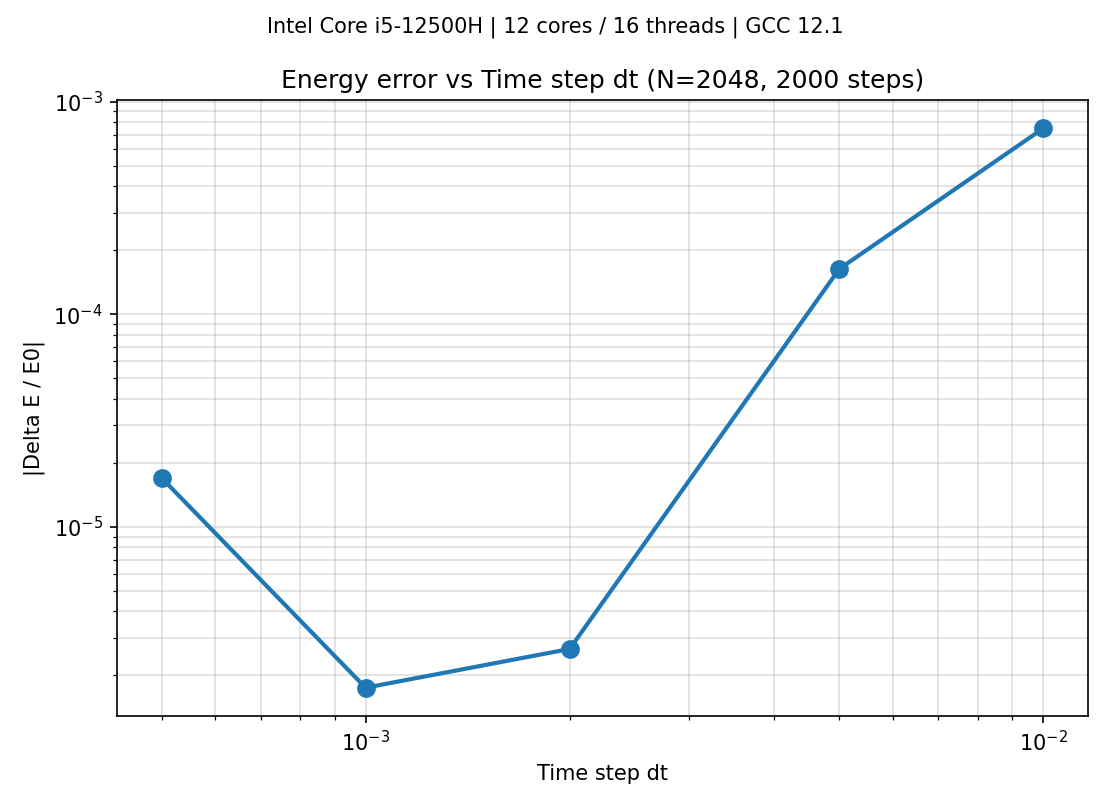
\includegraphics[width=0.85\linewidth]{vvduong_energy_dt}
\caption{Độ lệch năng lượng $|\Delta E/E_0|$ theo $\Delta t$ ($\varepsilon=0.01$).}
\label{fig:vvduong_energy_dt}
\end{figure}

\begin{figure}[H]
\centering
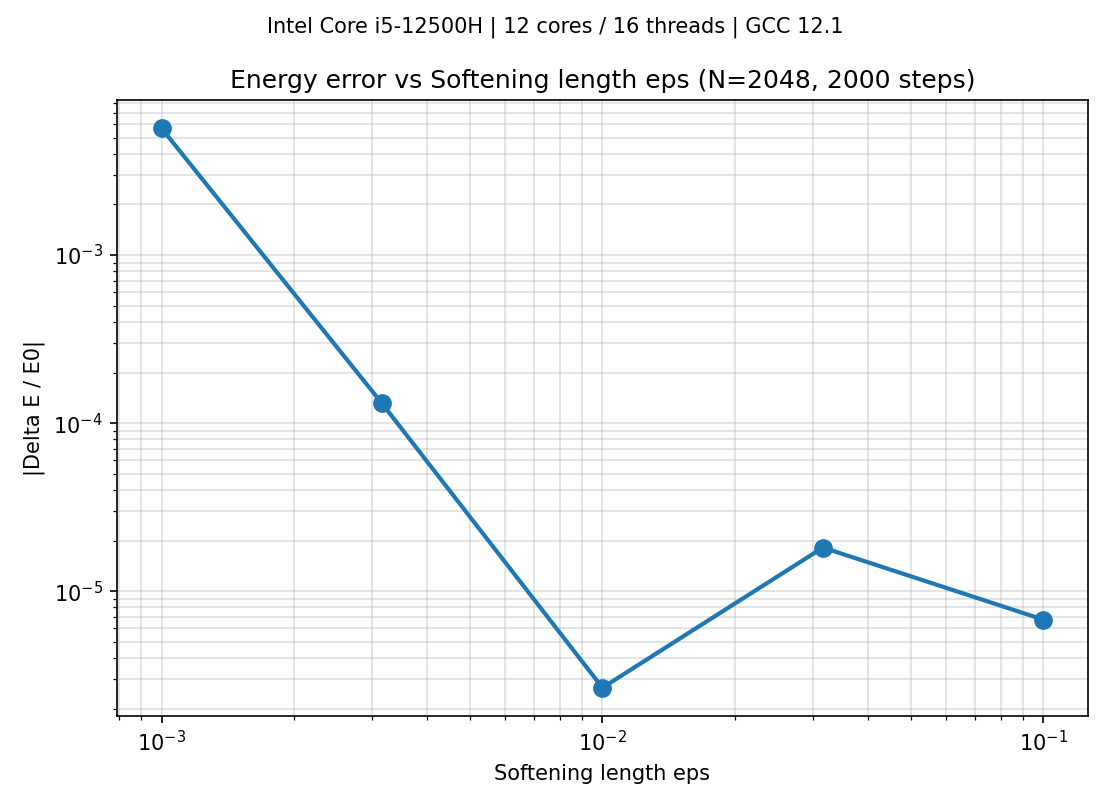
\includegraphics[width=0.85\linewidth]{vvduong_energy_eps}
\caption{Độ lệch năng lượng $|\Delta E/E_0|$ theo $\varepsilon$ ($\Delta t=0.002$).}
\label{fig:vvduong_energy_eps}
\end{figure}

Dữ liệu thô, gồm cả cấu hình máy và tham số từng lần chạy, nằm trong tệp\\ \code{results/vvduong\_energy.csv}.

Khi tăng $\Delta t$ từ 0.002 lên 0.005 và 0.01, độ lệch năng lượng cuối tăng từ $2.685\times10^{-6}$ lên $9.308\times10^{-5}$ và $1.260\times10^{-3}$. Kết quả ở $\Delta t=0.0005$ không nhỏ hơn mọi giá trị khác: $1.700\times10^{-5}$, lớn hơn các giá trị tại 0.001 và 0.002. Điều này cho thấy độ lệch tại một thời điểm cuối không nhất thiết đơn điệu theo bước thời gian; năng lượng của tích phân symplectic có thể dao động và kết quả còn phụ thuộc pha tại thời điểm đo.

Trong phép quét softening, $\varepsilon=0.001$ cho độ lệch lớn nhất $4.799\times10^{-3}$, trong khi $\varepsilon=0.01$ cho $2.685\times10^{-6}$. Các điểm còn lại không tạo thành xu hướng đơn điệu. $\varepsilon$ nhỏ làm lực ở cự ly gần nhạy hơn, còn $\varepsilon$ lớn làm thay đổi đáng kể mô hình thế năng; vì vậy không thể suy ra một quy luật đơn giản chỉ từ một seed và một thời điểm cuối.

\textbf{Giới hạn của phép so sánh:} mỗi lần chạy dùng cùng 2000 bước. Vì vậy, khi thay đổi $\Delta t$, tổng thời gian vật lý $T=2000\Delta t$ cũng thay đổi (từ 1 đến 20 đơn vị thời gian). Các số liệu \texttt{dt} mô tả đúng cấu hình thí nghiệm đã chạy nhưng chưa phải phép so sánh sai số tại cùng một thời điểm vật lý. Một khảo sát hội tụ chặt chẽ hơn cần giữ $T$ cố định và điều chỉnh số bước tỷ lệ nghịch với $\Delta t$. Ngược lại, trong phép quét \texttt{eps}, $\Delta t$ không đổi nên tổng thời gian mô phỏng bằng nhau.

\subsection{Quỹ đạo mô phỏng}

Quỹ đạo được tạo với $N=1024$, 2000 bước, $\Delta t=0.002$, $\varepsilon=0.01$, lưu trạng thái mỗi 20 bước. Hình~\ref{fig:vvduong_energy_orbit} so sánh trạng thái ban đầu và trạng thái ở bước 2000: cụm sao giữ cấu trúc cầu với lõi đặc ở tâm, phù hợp với một cụm Plummer ở trạng thái cân bằng. Ảnh động toàn bộ quỹ đạo (101 khung hình) nằm trong tệp \code{results/vvduong\_energy\_orbit.gif}.

\begin{figure}[H]
\centering
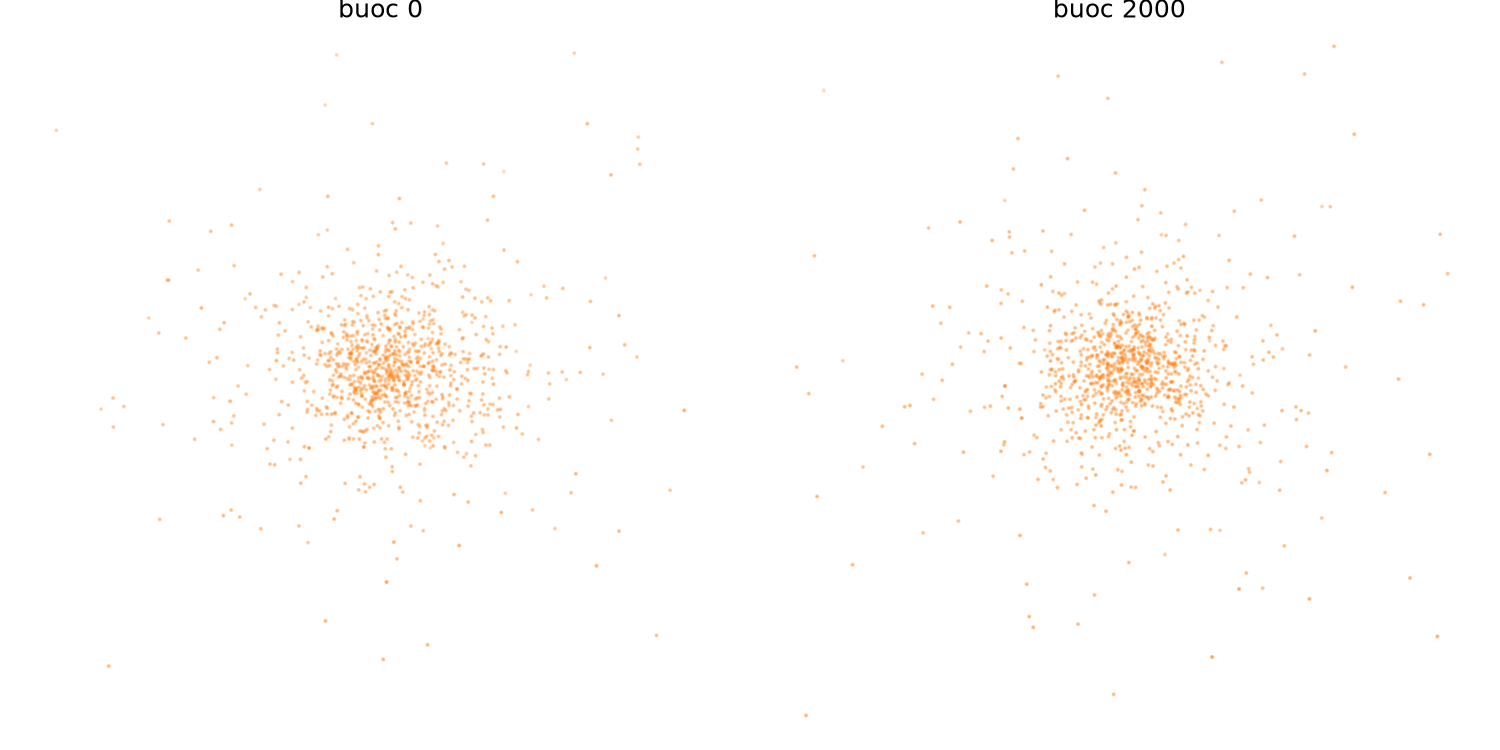
\includegraphics[width=0.85\linewidth]{vvduong_energy_orbit}
\caption{Cụm sao Plummer ở bước 0 và bước 2000 ($N=1024$).}
\label{fig:vvduong_energy_orbit}
\end{figure}

\section{Song song hóa trên CPU bằng OpenMP}
\label{sec:cai-dat-openmp}

\subsection{Cài đặt}

\subsubsection{Chia vòng lặp ngoài}
Theo chiến lược ở Mục~\ref{sec:chien-luoc}, chỉ thị \code{\#pragma omp parallel for}~\cite{openmp52} được đặt trên vòng lặp ngoài $i$ của pha tính gia tốc (Hình~\ref{fig:tuan-tu}); mỗi luồng nhận một đoạn chỉ số $i$ và tính trọn tổng theo $j$ cho các vật thể đó:
\begin{lstlisting}[language=C]
static void nb_acc_omp(const vec4f *pos, vec4f *acc, int n, float eps2)
{
    int i;
#pragma omp parallel for schedule(static) num_threads(nb_num_threads())
    for (i = 0; i < n; i++) nb_body_acc(pos, acc, i, n, eps2);
}
\end{lstlisting}

\subsubsection{Không có xung đột dữ liệu}
Như đã phân tích ở Mục~\ref{sec:phan-tich-nbody}, phân rã theo vật thể đích không gây xung đột dữ liệu. Cụ thể, trong \code{nb\_acc\_omp}:
\begin{itemize}
\item \textbf{Dữ liệu đọc (\texttt{read-only}):} Mảng tọa độ \texttt{pos} chứa vị trí và khối lượng của tất cả các hạt được đọc bởi tất cả các luồng. Không có luồng nào ghi vào \texttt{pos} trong quá trình tính gia tốc.
\item \textbf{Dữ liệu ghi (\texttt{write-private}):} Mỗi vật thể $i$ được gán cố định cho duy nhất một luồng phụ trách. Luồng tính toán gia tốc $\mathbf{a}_i$ và chỉ ghi kết quả vào phần tử \texttt{acc[i]} của riêng nó.
\item \textbf{Kết luận:} Mọi luồng hoạt động trên các địa chỉ bộ nhớ độc lập nhau ở mảng đích. Do đó, \textbf{hoàn toàn không có xung đột dữ liệu}, loại bỏ hoàn toàn nhu cầu sử dụng các cơ chế đồng bộ nặng nề như \texttt{\#pragma omp critical} hay \texttt{\#pragma omp atomic}.
\end{itemize}

\subsubsection{Vector hóa mức lệnh với \texttt{\#pragma omp simd}}
Bên trong hàm tính gia tốc hạt \texttt{nb\_body\_acc}, vòng lặp trong theo $j$ duyệt qua các phần tử liên tục trong bộ nhớ. Ta áp dụng chỉ thị vector hóa SIMD:
\begin{lstlisting}[language=C]
#pragma omp simd reduction(+ : ax, ay, az)
for (j = 0; j < n; j++) {
    const float dx = pos[j].x - xi;
    const float dy = pos[j].y - yi;
    const float dz = pos[j].z - zi;
    const float d2 = dx * dx + dy * dy + dz * dz + eps2;
    const float inv = 1.0f / sqrtf(d2);
    const float s = pos[j].w * inv * inv * inv;
    ax += dx * s;
    ay += dy * s;
    az += dz * s;
}
\end{lstlisting}
Nhờ chỉ thị này, trình biên dịch GCC sinh mã sử dụng các tập thanh ghi vector AVX2 (256-bit, chứa 8 số thực \texttt{float}) và tập lệnh FMA (Fused Multiply-Add). Các biến tích lũy \texttt{ax, ay, az} được thực hiện thông qua toán tử rút gọn \texttt{reduction(+)}, giúp CPU tính toán song song dữ liệu trong cùng một lõi vật lý.

\subsubsection{Khởi động nhóm luồng trước khi đo}
Lần đầu gặp vùng song song, runtime OpenMP phải tạo nhóm luồng và bộ đệm còn trống (cache cold miss). Nếu tính cả chi phí này, kết quả đo bị sai lệch, nhất là khi $N$ nhỏ. Vì vậy chương trình gọi một lần tính gia tốc để khởi động (\emph{warm-up}) trước khi bấm giờ:
\begin{lstlisting}[language=C]
if (parallel) nb_acc_omp(pos, acc, n, eps2);  // warm-up, không tính giờ
\end{lstlisting}

\subsection{Speedup và hiệu suất theo số luồng}

Thí nghiệm đo trên Intel Core i7-13620H (6 lõi P + 4 lõi E, 16 luồng), mỗi cấu hình chạy 3 lần lấy giá trị tốt nhất. Speedup $S_p$ và hiệu suất $E_p$ tính theo \eqref{eq:speedup}, với $T_1$ là thời gian bản tuần tự (Bảng~\ref{tab:omp-threads}, Hình~\ref{fig:ntduong_threads_speedup}).

\begin{table}[!htbp]
\centering\small
\setlength{\tabcolsep}{4pt}
\begin{tabular}{ccccccc}
\toprule
\textbf{$N$} & \textbf{Số luồng ($p$)} & \textbf{Thời gian (s)} & \textbf{ms/bước} & \textbf{GFLOP/s} & \textbf{$S_p$} & \textbf{$E_p$} \\
\midrule
\textbf{2048} & Tuần tự (1T) & 0.011936 & 2.387 & 35.14 & 1.00× & 100.0\% \\
2048 & 1 & 0.012060 & 2.412 & 34.78 & 0.99× & 99.0\% \\
2048 & 2 & 0.006315 & 1.263 & 66.42 & 1.89× & 94.5\% \\
2048 & 4 & 0.003471 & 0.694 & 120.85 & 3.44× & 86.0\% \\
2048 & 8 & 0.003398 & 0.680 & 123.42 & 3.51× & 43.9\% \\
2048 & 16 & 0.003399 & 0.680 & 123.41 & 3.51× & 21.9\% \\
\textbf{4096} & Tuần tự (1T) & 0.046801 & 9.360 & 35.85 & 1.00× & 100.0\% \\
4096 & 1 & 0.047925 & 9.585 & 35.01 & 0.98× & 97.7\% \\
4096 & 2 & 0.024209 & 4.842 & 69.30 & 1.93× & 96.7\% \\
4096 & 4 & 0.012909 & 2.582 & 129.96 & 3.63× & 90.6\% \\
4096 & 8 & 0.014544 & 2.909 & 115.36 & 3.22× & 40.2\% \\
4096 & 16 & 0.012868 & 2.574 & 130.38 & 3.64× & 22.7\% \\
\textbf{8192} & Tuần tự (1T) & 0.197202 & 39.440 & 34.03 & 1.00× & 100.0\% \\
8192 & 1 & 0.193234 & 38.647 & 34.73 & 1.02× & 102.1\% \\
8192 & 2 & 0.096843 & 19.369 & 69.30 & 2.04× & 101.8\% \\
8192 & 4 & 0.050336 & 10.067 & 133.32 & 3.92× & 97.9\% \\
8192 & 8 & 0.044343 & 8.869 & 151.34 & 4.45× & 55.6\% \\
8192 & 16 & \textbf{0.033364} & \textbf{6.673} & \textbf{201.14} & \textbf{5.91×} & \textbf{36.9\%} \\
\textbf{16384} & Tuần tự (1T) & 0.773194 & 154.639 & 34.72 & 1.00× & 100.0\% \\
16384 & 1 & 0.786256 & 157.251 & 34.14 & 0.98× & 98.3\% \\
16384 & 2 & 0.455911 & 91.182 & 58.88 & 1.70× & 84.8\% \\
16384 & 4 & 0.241187 & 48.237 & 111.30 & 3.21× & 80.1\% \\
16384 & 8 & 0.165322 & 33.064 & 162.37 & 4.68× & 58.5\% \\
16384 & 16 & \textbf{0.138587} & \textbf{27.717} & \textbf{193.69} & \textbf{5.58×} & \textbf{34.9\%} \\
\bottomrule
\end{tabular}
\caption{Speedup và hiệu suất OpenMP theo số luồng (i7-13620H, 5 bước).}
\label{tab:omp-threads}
\end{table}

\begin{figure}[H]
\centering
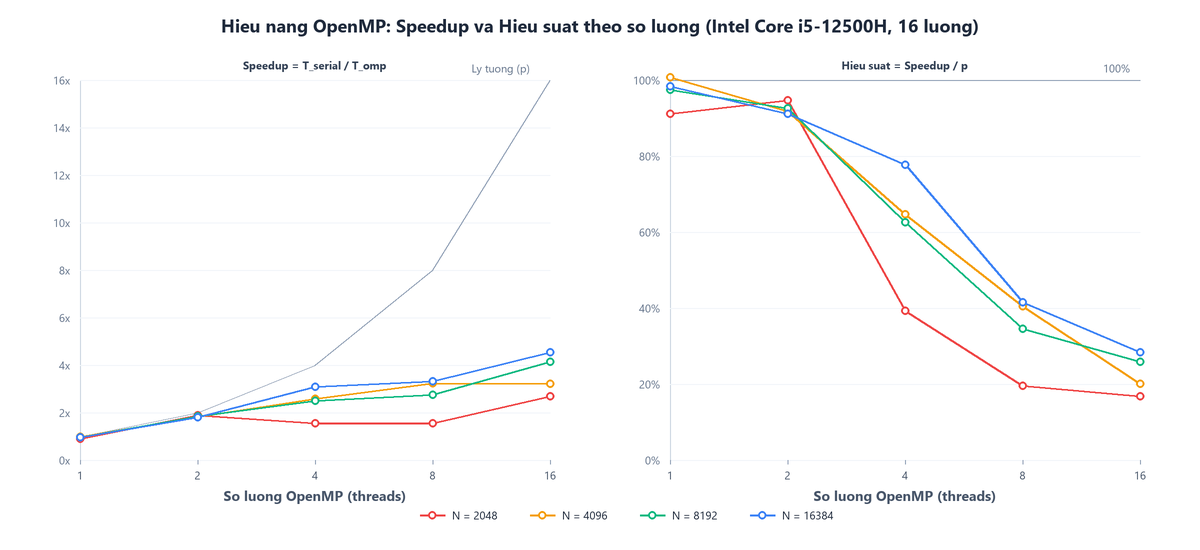
\includegraphics[width=0.85\linewidth]{ntduong_threads_speedup}
\caption{Speedup và hiệu suất OpenMP theo số luồng.}
\label{fig:ntduong_threads_speedup}
\end{figure}

\subsubsection{Vì sao speedup thấp hơn mức lý tưởng 16 lần}

Từ số liệu thực nghiệm, ta thấy Speedup tăng trưởng gần như tuyến tính tuyệt đối từ 1 đến 4 luồng ($S_2 \approx 1.93\times - 2.04\times$, $S_4 \approx 3.44\times - 3.92\times$, hiệu suất $86\% - 100\%$). Tuy nhiên, khi tăng lên 8 và 16 luồng, mức tăng tốc bắt đầu chậm lại và đạt đỉnh ở \textbf{5.91×} ($N=8192$, hiệu năng 201 GFLOP/s).

Hiện tượng này không phải do cài đặt sai mà bắt nguồn từ các đặc tính kiến trúc phần cứng máy tính hiện đại:

\begin{enumerate}
\item \textbf{Kiến trúc nhân bất đối xứng (Heterogeneous Core Topology):}
\begin{itemize}
\item Vi xử lý Intel Core i7-13620H gồm 10 lõi vật lý: 6 lõi P và 4 lõi E.
\item Sáu lõi P hỗ trợ Hyper-Threading (mỗi lõi 2 luồng logic) $\rightarrow$ 12 luồng logic.
\item Bốn lõi E không có Hyper-Threading $\rightarrow$ 4 luồng logic. Tổng cộng là 16 luồng.
\item Khi chạy từ 1 đến 4 luồng, hệ điều hành ưu tiên cấp phát trên 4 lõi P vật lý riêng biệt, nên mỗi luồng độc chiếm toàn bộ tài nguyên tính toán FMA/AVX2 $\rightarrow$ Hiệu suất đạt gần 100\%.
\item Khi chạy 16 luồng, các luồng phải chia sẻ nhân thực (Hyper-Threading trên P-core phải dùng chung các đơn vị thực thi FPU/ALU) và 4 luồng chạy trên E-core có xung nhịp và năng lực tính toán dấu phẩy động thấp hơn đáng kể. Do đó, mức tăng tốc không thể đạt 16×.

\end{itemize}
\item \textbf{Cơ chế giảm xung nhịp Turbo Boost do giới hạn nhiệt và điện năng (Power Throttling):}
\begin{itemize}
\item Khi chạy 1 luồng đơn tuần tự, CPU có thể đẩy xung nhịp của 1 nhân P lên mức tối đa \textbf{4.90 GHz}.
\item Khi chạy đồng thời 16 luồng ở cường độ tính toán AVX2 cao, để giữ công suất tiêu thụ dưới giới hạn gói TDP (45W - 115W), vi xử lý tự động hạ xung nhịp toàn nhân xuống còn khoảng \textbf{2.80 GHz - 3.20 GHz}.
\item Do xung nhịp cơ sở của mỗi nhân khi chạy đa luồng giảm đi khoảng $35\% - 40\%$ so với khi chạy đơn luồng, Speedup đo được tính trên thời gian tuần tự của nhân boost 4.9 GHz sẽ luôn thấp hơn tỷ lệ số luồng thuần túy.

\end{itemize}
\item \textbf{Nghẽn băng thông bộ nhớ (Memory Bandwidth Bottleneck) ở $N$ lớn:}
\begin{itemize}
\item Với $N=16384$, mảng vị trí \texttt{pos} có kích thước $256\text{ KB}$. Mặc dù nằm trong L2/L3 cache, nhưng 16 luồng liên tục đọc đồng thời từ hàng triệu vòng lặp gây áp lực lớn lên các cổng nạp của bộ nhớ đệm (L1/L2 read ports) và bus kết nối liên lõi (Ring Bus).

\end{itemize}
\item \textbf{Kích thước bài toán quá nhỏ khi $N=2048$ và $4096$:}
\begin{itemize}
\item Với $N=2048$, thời gian chạy ở 4 luồng chỉ mất \textbf{0.0035 giây (3.5 ms)}. Ở khoảng thời gian cực ngắn này, chi phí khởi tạo, chuyển ngữ cảnh và đồng bộ luồng tại barrier bắt đầu lấn át thời gian tính toán thực, khiến việc tăng lên 8 hay 16 luồng không làm giảm thêm thời gian thực thi.
\end{itemize}
\end{enumerate}

Đối chiếu với định luật Amdahl \eqref{eq:amdahl}: phần tuần tự của chương trình rất nhỏ khi $N$ lớn, nên giới hạn speedup ở đây không đến từ phần tuần tự mà từ phần cứng: các luồng không có năng lực tính như nhau và cùng tranh chấp tài nguyên chung. Đây là những yếu tố mà mô hình Amdahl lý tưởng không xét đến.

\subsection{Lập lịch và vector hóa SIMD}

Thí nghiệm này so sánh ba chế độ \code{schedule} (Mục~\ref{sec:openmp}) khi bật và tắt vector hóa SIMD, cùng máy i7-13620H, MinGW-W64 GCC 16.2.0 với cờ \code{-O3 -march=native -ffast-math -fopenmp}, 16 luồng, mỗi cấu hình chạy 3 lần lấy kết quả tốt nhất (Bảng~\ref{tab:schedule-simd}).

\begin{table}[H]
\centering\small
\begin{tabular}{cccccc}
\toprule
\textbf{$N$} & \textbf{Schedule} & \textbf{SIMD} & \textbf{ms/bước} & \textbf{GFLOP/s} & \textbf{Tăng tốc SIMD} \\
\midrule
\textbf{2048} & \texttt{static} & \textbf{ON} & \textbf{0.546} & \textbf{153.54} & \textbf{2.50×} \\
2048 & \texttt{static} & OFF & 1.365 & 61.45 & 1.00× \\
2048 & \texttt{dynamic,64} & \textbf{ON} & \textbf{0.581} & \textbf{144.36} & \textbf{1.93×} \\
2048 & \texttt{dynamic,64} & OFF & 1.123 & 74.71 & 1.00× \\
2048 & \texttt{guided,64} & \textbf{ON} & \textbf{0.567} & \textbf{147.92} & \textbf{2.06×} \\
2048 & \texttt{guided,64} & OFF & 1.169 & 71.79 & 1.00× \\
\textbf{4096} & \texttt{static} & \textbf{ON} & \textbf{2.103} & \textbf{159.54} & \textbf{1.88×} \\
4096 & \texttt{static} & OFF & 3.947 & 85.02 & 1.00× \\
4096 & \texttt{dynamic,64} & \textbf{ON} & \textbf{1.586} & \textbf{211.55} & \textbf{2.39×} \\
4096 & \texttt{dynamic,64} & OFF & 3.783 & 88.71 & 1.00× \\
4096 & \texttt{guided,64} & \textbf{ON} & \textbf{1.797} & \textbf{186.73} & \textbf{2.03×} \\
4096 & \texttt{guided,64} & OFF & 3.648 & 91.98 & 1.00× \\
\textbf{8192} & \texttt{static} & \textbf{ON} & \textbf{7.119} & \textbf{188.54} & \textbf{2.09×} \\
8192 & \texttt{static} & OFF & 14.867 & 90.28 & 1.00× \\
8192 & \texttt{dynamic,64} & \textbf{ON} & \textbf{5.849} & \textbf{229.46} & \textbf{2.38×} \\
8192 & \texttt{dynamic,64} & OFF & 13.930 & 96.35 & 1.00× \\
8192 & \texttt{guided,64} & \textbf{ON} & \textbf{6.437} & \textbf{208.51} & \textbf{2.21×} \\
8192 & \texttt{guided,64} & OFF & 14.243 & 94.23 & 1.00× \\
\textbf{16384} & \texttt{static} & \textbf{ON} & \textbf{26.136} & \textbf{205.42} & \textbf{2.19×} \\
16384 & \texttt{static} & OFF & 57.268 & 93.75 & 1.00× \\
16384 & \texttt{dynamic,64} & \textbf{ON} & \textbf{23.148} & \textbf{231.93} & \textbf{2.37×} \\
16384 & \texttt{dynamic,64} & OFF & 54.891 & 97.81 & 1.00× \\
16384 & \texttt{guided,64} & \textbf{ON} & \textbf{25.437} & \textbf{211.06} & \textbf{2.26×} \\
16384 & \texttt{guided,64} & OFF & 57.507 & 93.36 & 1.00× \\
\bottomrule
\end{tabular}
\caption{Thời gian và hiệu năng theo chế độ lập lịch, bật/tắt SIMD (i7-13620H, 16 luồng).}
\label{tab:schedule-simd}
\end{table}

\begin{figure}[H]
\centering
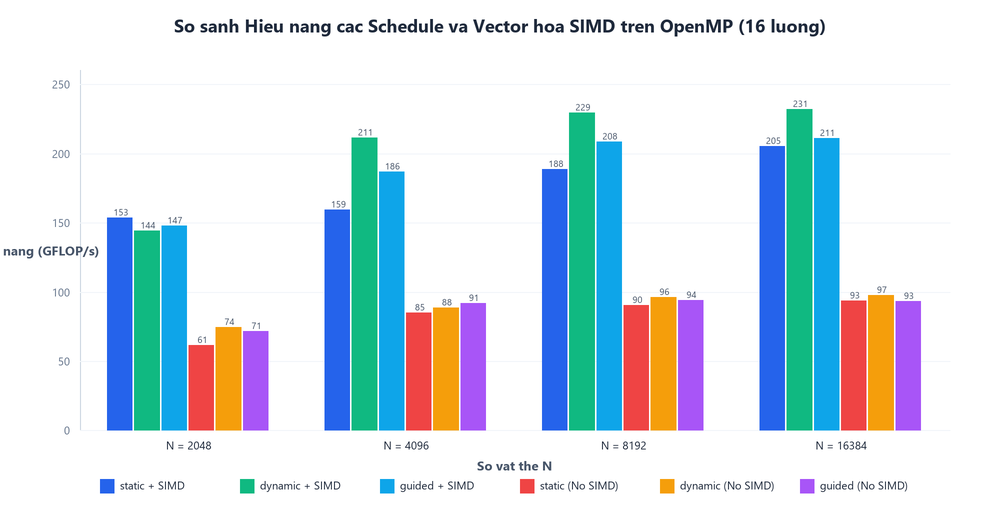
\includegraphics[width=0.85\linewidth]{ntduong_schedule_simd}
\caption{So sánh các chế độ schedule, có và không có SIMD (16 luồng).}
\label{fig:ntduong_schedule_simd}
\end{figure}

\subsubsection{Phân tích}

\begin{enumerate}
\item \textbf{Hiệu ứng vượt trội của SIMD:}
\begin{itemize}
\item Trên tất cả các giá trị $N$, việc bật SIMD (\texttt{\#pragma omp simd reduction}) đem lại mức tăng tốc \textbf{1.88× đến 2.50×} (đạt \textbf{2.09× đến 2.38×} ở $N = 8192\text{--}16384$) so với bản vô hướng không có SIMD.
\item Lưu ý: với \code{-O3 -ffast-math}, GCC tự vector hóa, nên bản OFF (hàm \code{nb\_body\_acc\_nosimd}) được đánh dấu \code{\_\_attribute\_\_((optimize("no-tree-vectorize")))} để đo đúng bản vô hướng. Kiểm tra bằng \code{-fopt-info-vec} cho thấy hàm này không còn vòng lặp nào được vector hóa. Tốc độ bản vô hướng thật (khoảng 90--98 GFLOP/s ở $N = 8192\text{--}16384$) xấp xỉ bản trước khi thêm thuộc tính này, vì ở bản cũ trình biên dịch tự vector hóa với hệ số mở vòng 32, gây tràn thanh ghi YMM ra bộ nhớ ngăn xếp và làm hiệu năng giảm xuống ngang mức vô hướng.
\item Lý do: vòng lặp $j$ của bản SIMD ON được dịch thành lệnh AVX2 256 bit (\code{vrsqrtps}), xử lý 8 tương tác trong một lệnh thay vì từng số vô hướng (\code{vsqrtss}, \code{vmulss}, \code{vdivss}).

\end{itemize}
\item \textbf{Hiện tượng bất đối xứng trên kiến trúc CPU lai (Hybrid P/E Cores):}
\begin{itemize}
\item Theo lý thuyết tính toán song song truyền thống, bài toán All-Pairs có khối lượng mỗi vòng lặp ngoài $i$ là hoàn toàn đồng đều ($N$ tương tác), nên \texttt{schedule(static)} được xem là tối ưu vì chi phí lập lịch bằng 0.
\item Tuy nhiên, số liệu thực nghiệm trên vi xử lý Intel Core i7-13620H lại chỉ ra: \textbf{\texttt{schedule(dynamic, 64)} nhanh hơn \texttt{schedule(static)} rõ rệt} (với $N=16384$, \texttt{dynamic} đạt \textbf{231.93 GFLOP/s}, trong khi \texttt{static} đạt \textbf{205.42 GFLOP/s} — chênh lệch \textasciitilde{}13\%; và với $N=4096\text{--}8192$ đạt \textbf{211.55–229.46 GFLOP/s}, nhanh hơn \texttt{static} tới 21\%–33\%).
\item \textbf{Giải thích cơ chế vật lý:} CPU Intel thế hệ 13 sở hữu 2 loại lõi khác nhau:
\begin{itemize}
\item 6 lõi P (Performance Core): Kiến trúc Raptor Cove, IPC cao, xung nhịp Turbo lên tới 4.9 GHz.
\item 4 lõi E (Efficient Core): Kiến trúc Gracemont, IPC thấp hơn, xung nhịp tối đa chỉ 3.6 GHz.
\item Với \texttt{schedule(static)}, công việc được chia đều thành các đoạn $N/16$. Các luồng chạy trên nhân P-core tính xong sớm hơn nhiều nhưng buộc phải \textbf{chờ đợi (idle wait)} tại rào đồng bộ ngầm của OpenMP để các luồng chạy trên nhân E-core chậm hơn hoàn thành.
\item Với \texttt{schedule(dynamic, 64)}, các nhân P-core sau khi hoàn thành phần của mình sẽ tiếp tục tranh thủ nhận các gói 64 hạt tiếp theo từ hàng đợi chung, giúp toàn bộ hệ thống đạt độ cân bằng tải tối ưu nhất.
\end{itemize}
\end{itemize}
\end{enumerate}

\subsection{Biến thể dùng định luật 3 Newton}

\subsubsection{Ý tưởng và vấn đề xung đột dữ liệu}
Định luật 3 Newton phát biểu rằng lực tác dụng giữa hai vật là trực đối: $\mathbf{F}_{ji} = -\mathbf{F}_{ij}$. Do đó, ta chỉ cần duyệt qua các cặp $(i, j)$ với $i < j$, giảm số phép tính từ $N^2$ xuống còn:
\[ \frac{N(N-1)}{2} \approx \frac{N^2}{2} \text{ cặp tương tác} \]

Tuy nhiên, khi luồng tính toán tương tác giữa cặp $(i, j)$, nó phải cập nhật đồng thời gia tốc cho cả hai vật thể:
\[ \Delta \mathbf{a}_i = + m_j \frac{\mathbf{r}_{ij}}{\left(|\mathbf{r}_{ij}|^2 + \varepsilon^2\right)^{3/2}}, \quad \Delta \mathbf{a}_j = - m_i \frac{\mathbf{r}_{ij}}{\left(|\mathbf{r}_{ij}|^2 + \varepsilon^2\right)^{3/2}} \]

Nếu hai luồng khác nhau cùng tương tác với cùng một vật thể $j$ tại một thời điểm, \textbf{Race Condition sẽ xảy ra} và làm sai lệch nghiêm trọng kết quả.

\subsubsection{Giải pháp: mảng đệm riêng cho từng luồng}
Để song song hóa mà không dùng khóa tuần tự hóa (\texttt{atomic}/\texttt{critical}), ta cấp phát cho mỗi luồng $t \in [0, p-1]$ một mảng đệm gia tốc riêng biệt:
\begin{lstlisting}[language=C]
// mỗi luồng có một mảng đệm \code{my\_acc} gồm N phần tử
vec4f *my_acc = acc_threads + (size_t)tid * (size_t)n;
\end{lstlisting}
Trong vòng lặp song song:
\begin{itemize}
\item Luồng $tid$ chỉ cộng dồn vào \texttt{my\_acc[i]} và \texttt{my\_acc[j]} của riêng nó.
\item Sau khi kết thúc duyệt tất cả các cặp, ta thực hiện bước \textbf{Reduction} (cộng dồn $p$ mảng cục bộ vào mảng \texttt{acc} chung) theo cách song song hóa:
\end{itemize}
\begin{lstlisting}[language=C]
#pragma omp for schedule(static)
for (i = 0; i < n; i++) {
    float sx = 0.0f, sy = 0.0f, sz = 0.0f;
    for (int t = 0; t < p; t++) {
        sx += acc_threads[(size_t)t * n + i].x;
        sy += acc_threads[(size_t)t * n + i].y;
        sz += acc_threads[(size_t)t * n + i].z;
    }
    acc[i].x = sx; acc[i].y = sy; acc[i].z = sz;
}
\end{lstlisting}

\subsubsection{Kết quả đo: all-pairs và Newton 3}

\begin{table}[H]
\centering\small
\begin{tabular}{ccccc}
\toprule
\textbf{$N$} & \textbf{Số luồng} & \textbf{All-pairs (ms/bước)} & \textbf{Newton 3 (ms/bước)} & \textbf{All-pairs nhanh hơn} \\
\midrule
2048 & 1 & 2.427 & 3.352 & 1.38× \\
2048 & 4 & 0.726 & 1.631 & 2.25× \\
2048 & 16 & 0.885 & 1.086 & 1.23× \\
4096 & 1 & 9.506 & 13.899 & 1.46× \\
4096 & 4 & 2.900 & 6.214 & 2.14× \\
4096 & 16 & 2.076 & 2.826 & 1.36× \\
8192 & 1 & 38.813 & 54.367 & 1.40× \\
8192 & 4 & 11.829 & 24.445 & 2.07× \\
8192 & 16 & 7.745 & 11.227 & 1.45× \\
16384 & 1 & 158.180 & 221.712 & 1.40× \\
16384 & 4 & 43.871 & 98.553 & 2.25× \\
16384 & 8 & 31.526 & 60.997 & 1.93× \\
16384 & 16 & \textbf{25.537} & \textbf{41.603} & \textbf{1.63×} \\
\bottomrule
\end{tabular}
\caption{So sánh thời gian all-pairs và biến thể định luật 3 Newton (i7-13620H).}
\label{tab:newton3}
\end{table}

\begin{figure}[H]
\centering
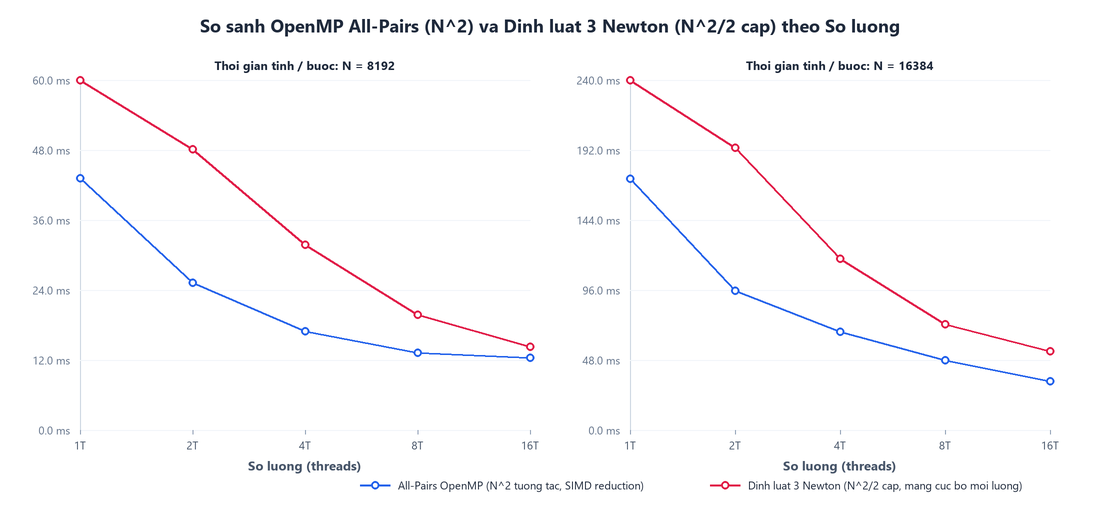
\includegraphics[width=0.85\linewidth]{ntduong_newton3_comparison}
\caption{So sánh All-Pairs và biến thể định luật 3 Newton.}
\label{fig:ntduong_newton3_comparison}
\end{figure}

\subsubsection{Vì sao biến thể Newton 3 chậm hơn}

Mặc dù định luật 3 Newton giảm $50\%$ số phép toán, phiên bản này chạy \textbf{chậm hơn từ 1.2× đến 2.3×} so với all-pairs (Bảng~\ref{tab:newton3}). Kết quả này minh họa sự đánh đổi đã nêu ở Mục~\ref{sec:phan-tich-nbody}: giảm số phép tính nhưng phải trả giá bằng đồng bộ và truy cập bộ nhớ. Có bốn nguyên nhân chính:

\begin{enumerate}
\item \textbf{Mất khả năng vector hóa SIMD liên tục:}
\begin{itemize}
\item Trong All-Pairs, vòng lặp $j$ đọc tuần tự các phần tử liên tiếp từ \texttt{pos[j]} và tích lũy vào một biến thanh ghi cục bộ \texttt{ax, ay, az}. Trình biên dịch dễ dàng vector hóa bằng AVX2 FMA.
\item Trong Newton 3, vòng lặp phải ghi phân tán vào \texttt{my\_acc[j]} ở từng bước lặp. Do $j$ thay đổi, CPU phải thực hiện các thao tác ghi rải rác (\textbf{scatter writes}), triệt tiêu hoàn toàn khả năng vector hóa SIMD đơn giản.
\end{itemize}
\item \textbf{Áp lực bộ nhớ và suy hao Cache (Cache Thrashing):}
\begin{itemize}
\item Bản All-Pairs chỉ có mảng \texttt{pos} (chỉ đọc, nạp vào L2/L3 cache một lần và chia sẻ giữa mọi luồng) và \texttt{acc} ($N \times 16$ byte $\approx 256$ KB với $N=16384$, nằm gọn trong Cache L2).
\item Bản Newton 3 với 16 luồng cần $16 \times N \times 16$ byte $\approx \mathbf{4.19\text{ MB}}$ bộ nhớ ghi riêng. Mười sáu luồng liên tục ghi ngẫu nhiên vào các mảng đệm này, làm tràn bộ đệm L1/L2, đẩy mạnh tỷ lệ cache evictions và làm nghẽn bus bộ nhớ.
\end{itemize}
\item \textbf{Mất cân bằng tải do cấu trúc vòng lặp tam giác:}
\begin{itemize}
\item Do $j$ chạy từ $i+1$ đến $N$, các hạt có $i$ nhỏ cần tính gần $N$ tương tác, trong khi các hạt $i$ gần cuối chỉ cần tính vài tương tác. Dù đã dùng \texttt{schedule(guided)} hay \texttt{dynamic}, việc điều phối khối tam giác vẫn phát sinh overhead lớn hơn nhiều so với lưới chữ nhật đều của All-Pairs.
\end{itemize}
\item \textbf{Chi phí cộng dồn (Reduction Overhead):}
\begin{itemize}
\item Sau khi tính xong, hệ thống phải thực hiện thêm một vòng lặp duyệt $16 \times N$ phần tử để cộng dồn vào \texttt{acc}, tiêu tốn thêm thời gian và băng thông bộ nhớ.
\end{itemize}
\end{enumerate}

\subsection{Nhận xét về phiên bản OpenMP}

\begin{enumerate}
\item \textbf{Hiệu năng đạt được:}
\begin{itemize}
\item Phiên bản OpenMP All-Pairs đạt mức tăng tốc tối đa \textbf{5.91×} tại 16 luồng ($N=8192$), nâng hiệu năng tính toán CPU lên mức \textbf{201.14 GFLOP/s} (so với 34 GFLOP/s của bản tuần tự).
\item Kiểm tra tính đúng đắn (\texttt{-verify}) cho thấy kết quả song song khớp hoàn toàn từng bit với bản tuần tự (sai số tương đối $0.000\text{e}+00$), và năng lượng toàn phần được bảo toàn nghiêm ngặt ($|\Delta E / E_0| \approx 8.78 \times 10^{-7}$).
\end{itemize}
\item \textbf{Vai trò then chốt của SIMD:}
\begin{itemize}
\item Vector hóa SIMD thông qua \texttt{\#pragma omp simd reduction} mang lại mức cải thiện hiệu năng then chốt \textbf{1.9× đến 2.5×} so với bản vô hướng thực thụ (\texttt{no-tree-vectorize}), chứng minh tầm quan trọng của việc kết hợp đa luồng cấp lõi (multithreading) với song song hóa cấp lệnh (SIMD instruction-level parallelism).
\end{itemize}
\item \textbf{Bài học về lập lịch trên CPU lai:}
\begin{itemize}
\item Trên các dòng CPU kiến trúc lai hiện đại (Intel Core gen 12/13/14), \texttt{schedule(dynamic)} giúp cân bằng tải vượt trội giữa nhân P và nhân E, mang lại hiệu năng cao hơn \texttt{schedule(static)} từ \textbf{13\% đến 33\%} (tùy kích thước $N$).
\end{itemize}
\item \textbf{Bài học từ Định luật 3 Newton:}
\begin{itemize}
\item Việc giảm một nửa số phép tính toán học ($N^2/2$) không đồng nghĩa với việc tăng tốc độ thực tế. Chi phí bộ đệm cục bộ (4 MB), xung đột cache, mất vector hóa SIMD và chi phí reduction đã khiến bản Newton 3 chậm hơn bản All-Pairs tiêu chuẩn. Đây là minh chứng rõ ràng cho việc: \textbf{Trong tính toán hiện đại, cấu trúc dữ liệu thân thiện với bộ nhớ đệm (Cache-Friendly) và vector hóa SIMD quan trọng hơn số lượng phép tính thuần túy.}
\end{itemize}
\end{enumerate}

\section{Song song hóa trên GPU bằng CUDA}
\label{sec:cai-dat-cuda}

\subsection{Ánh xạ bài toán lên lưới luồng}

Theo chiến lược ở Mục~\ref{sec:chien-luoc}, \textbf{mỗi luồng CUDA phụ trách một vật thể đích} $i$. Tập $N$ vật thể được chia thành các khối một chiều, mỗi khối $B$ luồng ($B$ = \code{blockDim.x}). Số khối và chỉ số vật thể của mỗi luồng là:
\begin{equation}
\text{gridDim.x} = \left\lceil \frac{N}{B} \right\rceil = \frac{N+B-1}{B}, \qquad
i = \text{blockIdx.x} \times \text{blockDim.x} + \text{threadIdx.x}.
\end{equation}
Do số luồng có thể lớn hơn $N$, mỗi luồng kiểm tra $i<N$ trước khi tính. Mỗi luồng chỉ ghi \code{acc[i]} của mình nên không cần phép toán nguyên tử như \code{atomicAdd}. Chương trình khảo sát $B \in \{64, 128, 256, 512\}$.

Mảng vị trí được lưu dạng \code{float4} như trong GPU Gems 3~\cite{gpugems3}: ba thành phần $x,y,z$ là tọa độ, thành phần $w$ là khối lượng. Một bản ghi 16 byte giúp mỗi luồng đọc cả vị trí và khối lượng trong một lần truy cập. Dữ liệu được sao chép lên GPU một lần trước vòng lặp thời gian và chỉ chép về CPU ở cuối mô phỏng; mỗi bước gồm một kernel tính gia tốc và một kernel cập nhật trạng thái.

\subsection{Kernel naive}

Kernel naive là cách cài đặt trực tiếp: mỗi luồng đọc vị trí vật thể đích vào thanh ghi, rồi duyệt toàn bộ $N$ vật thể nguồn trong global memory để cộng gia tốc. Hàm \code{rsqrtf()} tính nghịch đảo căn bậc hai bằng đơn vị chức năng đặc biệt (SFU) của GPU.

\begin{lstlisting}[language=CUDA]
// Một tương tác (GPU Gems 3, Listing 31-1), khoảng 20 FLOP
__device__ float3 bodyBodyInteraction(float4 bi, float4 bj, float3 ai, float eps2) {
    float3 r = {bj.x - bi.x, bj.y - bi.y, bj.z - bi.z};
    float distSqr = r.x * r.x + r.y * r.y + r.z * r.z + eps2;
    float invDist = rsqrtf(distSqr);
    float s = bj.w * invDist * invDist * invDist;
    ai.x += r.x * s;  ai.y += r.y * s;  ai.z += r.z * s;
    return ai;
}

__global__ void accNaive(const float4 *pos, float4 *acc, int n, float eps2) {
    int i = blockIdx.x * blockDim.x + threadIdx.x;
    if (i >= n) return;
    float4 bi = pos[i];
    float3 a = make_float3(0.0f, 0.0f, 0.0f);
    for (int j = 0; j < n; j++)
        a = bodyBodyInteraction(bi, pos[j], a, eps2);   // pos[j] đọc từ global memory
    acc[i] = make_float4(a.x, a.y, a.z, 0.0f);
}
\end{lstlisting}

\textbf{Hạn chế về bộ nhớ.} Mỗi luồng đọc toàn bộ $N$ bản ghi 16 byte, nên tổng lưu lượng đọc theo mô hình trực tiếp là khoảng $16N^2$ byte, trong khi dữ liệu thực chỉ có $16N$ byte. Như đã phân tích ở Mục~\ref{sec:phan-tich-nbody}, cường độ tính toán khi đó chỉ khoảng $1.25$ FLOP/byte, thấp hơn nhiều so với điểm cân bằng $25.3$ FLOP/byte của T4, nên kernel có nguy cơ bị giới hạn bởi băng thông bộ nhớ. Trên thực tế bộ đệm L1/L2 giữ lại một phần dữ liệu đọc lặp, nhưng kernel naive vẫn phụ thuộc nhiều vào hệ thống bộ nhớ. Cần giảm số lần đọc global memory, và đó là mục tiêu của kernel tiled.

\subsection{Kernel tiled dùng shared memory}

\subsubsection{Ý tưởng}

Kernel tiled áp dụng kỹ thuật chia khối (\emph{tiling}) của GPU Gems 3~\cite{gpugems3}. Tập $N$ vật thể nguồn được chia thành $\lceil N/B \rceil$ \emph{tile}, mỗi tile $B$ vật thể (tile cuối có thể ít hơn). Với mỗi tile, $B$ luồng của một khối phối hợp nạp $B$ vị trí từ global memory vào shared memory, mỗi luồng nạp một phần tử; sau đó mỗi luồng dùng lại cả $B$ phần tử trong shared memory để cộng gia tốc cho vật thể đích của mình (Hình~\ref{fig:tiled}). Các luồng liền kề nạp các địa chỉ liền kề, nên các lần đọc được gộp (coalescing).

\begin{figure}[H]
\centering
\begin{tikzpicture}[>=Stealth, font=\small,
  box/.style={draw, minimum height=0.75cm, align=center},
  lab/.style={font=\footnotesize\itshape, align=center}]
  % global memory
  \node[lab, anchor=east] at (-0.2,3.6) {Global memory\\($N$ vị trí)};
  \foreach \k/\t in {0/Tile 0, 1/Tile 1, 2/Tile 2, 3/$\cdots$, 4/Tile $k$} {
    \node[box, minimum width=2cm, fill=black!5] (g\k) at (\k*2.1+1,3.6) {\t};
  }
  \node[box, minimum width=2cm, fill=orange!25] at (g2) {Tile 2};
  % shared memory
  \node[lab, anchor=east] at (-0.2,1.9) {Shared memory\\(một khối)};
  \node[box, minimum width=4.2cm, fill=orange!25] (sh) at (5.2,1.9) {\code{shPos[0 .. B-1]}};
  \draw[->, thick] (g2.south) -- node[right, lab] {$B$ luồng cùng nạp, mỗi luồng 1 phần tử} (sh.north);
  % threads
  \node[lab, anchor=east] at (-0.2,0.1) {Thanh ghi\\(mỗi luồng)};
  \foreach \k/\t in {0/Luồng 0, 1/Luồng 1, 2/$\cdots$, 3/Luồng $B-1$} {
    \node[box, minimum width=2cm, fill=blue!8] (t\k) at (\k*2.5+1.5,0.1) {\t};
    \draw[->] (sh.south) -- (t\k.north);
  }
  \node[lab] at (5.2,-0.9) {mỗi luồng đọc cả $B$ phần tử của tile, cộng dồn gia tốc cho vật thể $i$ của mình};
\end{tikzpicture}
\caption{Kernel tiled: một tile được nạp một lần cho cả khối rồi dùng lại $B$ lần.}
\label{fig:tiled}
\end{figure}

Theo mô hình lý tưởng, lượng dữ liệu nguồn đọc từ global memory giảm từ khoảng $N^2$ xuống $N^2/B$ phần tử, tức giảm $B$ lần, và cường độ tính toán tăng tương ứng (Mục~\ref{sec:phan-tich-nbody}). Hiệu quả thực tế còn phụ thuộc bộ đệm, chi phí đồng bộ và cách trình biên dịch tối ưu.

\subsubsection{Vòng lặp tile và hai lệnh \texttt{\_\_syncthreads()}}

\begin{lstlisting}[language=CUDA]
extern __shared__ float4 shPos[];          // B phần tử, cấp khi gọi kernel
const float4 bi = (i < n) ? pos[i] : make_float4(0, 0, 0, 0);
for (int tile = 0; tile * blockDim.x < n; tile++) {
    int j = tile * blockDim.x + threadIdx.x;
    shPos[threadIdx.x] = (j < n) ? pos[j] : make_float4(0, 0, 0, 0);
    __syncthreads();                       // (1) chờ cả khối nạp xong
#pragma unroll 8
    for (int k = 0; k < blockDim.x; k++)
        a = bodyBodyInteraction(bi, shPos[k], a, eps2);
    __syncthreads();                       // (2) chờ cả khối dùng xong
}
if (i < n) acc[i] = make_float4(a.x, a.y, a.z, 0.0f);
\end{lstlisting}

Kernel được gọi với kích thước shared memory động \code{B * sizeof(float4)} (tham số thứ ba trong \code{<<<grid, B, B*sizeof(float4)>>>}), nên cùng một mã chạy được với mọi $B$. Khác với kernel naive, luồng có $i \ge N$ \emph{không} được thoát sớm, vì mọi luồng của khối đều phải nạp tile và đi qua \code{\_\_syncthreads()}. Phần tử đệm ngoài phạm vi được gán khối lượng 0 nên đóng góp 0 vào gia tốc, không cần rẽ nhánh trong vòng trong. Hai lệnh đồng bộ có vai trò khác nhau và đều cần thiết~\cite{gpugems3}:
\begin{itemize}
\item \textbf{Lần (1) -- đọc sau ghi (RAW):} bảo đảm mọi luồng trong khối đã ghi xong phần tử của mình vào \code{shPos} trước khi bất kỳ luồng nào đọc \code{shPos[j]}. Thiếu lệnh này, một số warp có thể đọc dữ liệu chưa được nạp hoặc dữ liệu của tile cũ.
\item \textbf{Lần (2) -- ghi sau đọc (WAR):} bảo đảm không còn luồng nào đang đọc tile hiện tại trước khi tile tiếp theo được nạp đè lên cùng vùng nhớ. Thiếu lệnh này, warp chạy nhanh có thể ghi đè dữ liệu mà warp khác vẫn đang dùng.
\end{itemize}

\subsection{Kết quả trên Tesla T4}

Thí nghiệm chạy trên Google Colab: Tesla T4, driver 580.82.07, CUDA 13.0, \code{nvcc -O3}, số thực FP32; CPU của máy ảo là Intel Xeon 2.00 GHz, Linux 6.6. Phép so sánh naive--tiled dùng 5 bước, mỗi cấu hình đo 3 lần lấy lần nhanh nhất, $N$ từ 1024 đến 131072 và $B \in \{64,128,256,512\}$. Phép đo chi phí truyền dữ liệu dùng 10 bước, $B=256$.

\subsubsection{Kernel naive và tiled}

Bảng~\ref{tab:naive-tiled} cho thời gian 5 bước và hiệu năng của hai kernel với $B=256$; Hình~\ref{fig:gpu_speedup} so sánh speedup của OpenMP 16 luồng và hai kernel CUDA so với bản tuần tự (trục tung thang logarit).

\begin{table}[H]
\centering\small
\begin{tabular}{rrrrrr}
\toprule
\textbf{$N$} & \textbf{Naive (ms)} & \textbf{Tiled (ms)} & \textbf{Tiled/naive} & \textbf{GFLOP/s naive} & \textbf{GFLOP/s tiled} \\
\midrule
1024 & 0.315 & 0.205 & 1.54× & 332.54 & 511.52 \\
2048 & 0.625 & 0.391 & 1.60× & 670.93 & 1073.74 \\
4096 & 1.277 & 0.751 & 1.70× & 1313.48 & 2233.39 \\
8192 & 2.489 & 1.491 & 1.67× & 2696.09 & 4501.10 \\
16384 & 7.214 & 5.741 & 1.26× & 3720.98 & \textbf{4675.87} \\
32768 & 28.685 & 24.457 & 1.17× & 3743.21 & 4390.29 \\
65536 & 131.047 & 109.366 & 1.20× & 3277.41 & 3927.16 \\
131072 & 515.285 & 442.754 & 1.16× & 3334.05 & 3880.23 \\
\bottomrule
\end{tabular}
\caption{Thời gian 5 bước và hiệu năng của kernel naive và tiled trên Tesla T4 ($B=256$).}
\label{tab:naive-tiled}
\end{table}

\begin{figure}[H]
\centering
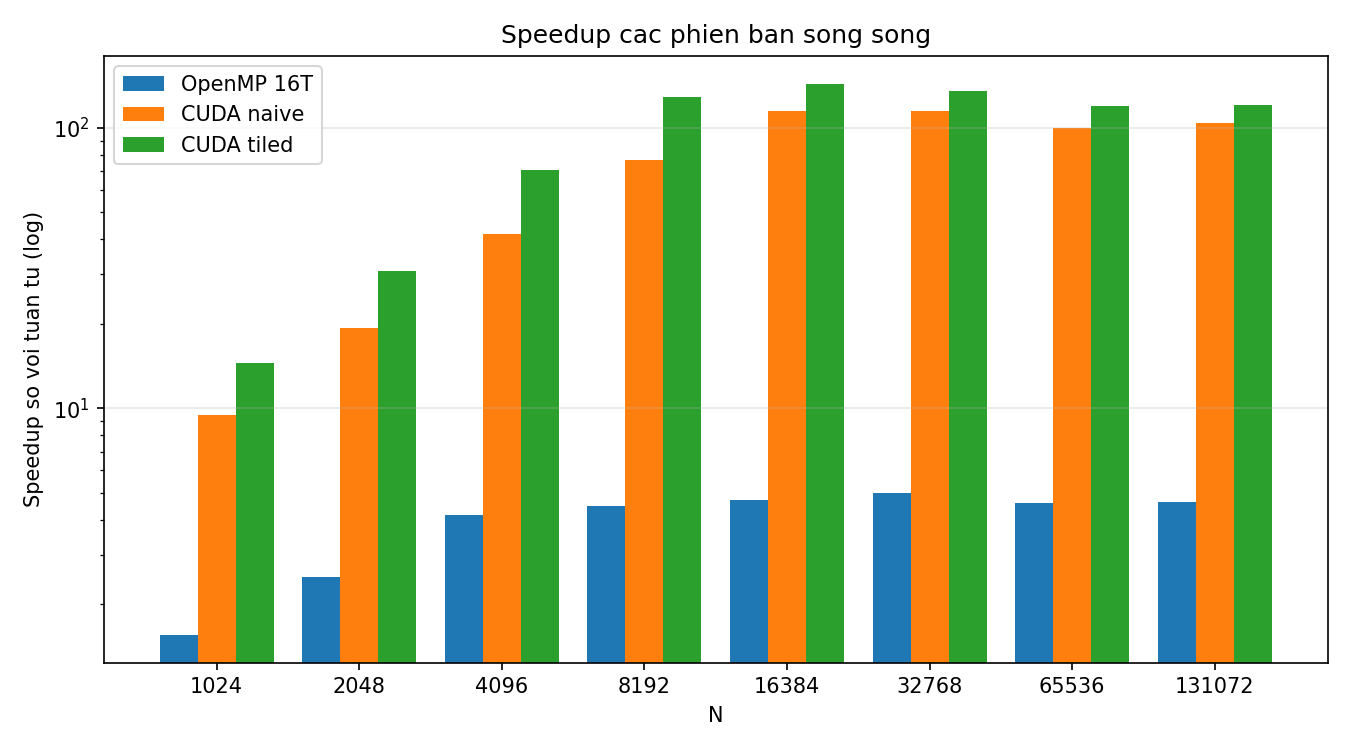
\includegraphics[width=0.85\linewidth]{gpu_speedup}
\caption{Speedup so với bản tuần tự của OpenMP 16 luồng, CUDA naive và CUDA tiled.}
\label{fig:gpu_speedup}
\end{figure}

Kernel tiled nhanh hơn naive ở mọi kích thước, từ 1.16 đến 1.70 lần. Lợi ích rõ nhất khi $N \le 8192$ (1.54--1.70 lần) nhờ tái sử dụng dữ liệu trong shared memory. Khi $N \ge 16384$, khoảng cách thu hẹp còn khoảng 1.2 lần: bộ đệm L1/L2 của Turing giữ lại phần lớn dữ liệu mà kernel naive đọc lặp, nên naive không còn bị giới hạn nặng bởi băng thông như mô hình lý tưởng dự đoán; trong khi đó tiled phải trả thêm chi phí nạp tile và đồng bộ.

\subsubsection{Ảnh hưởng của kích thước khối}

\begin{table}[H]
\centering\small
\begin{tabular}{rrrr}
\toprule
\textbf{$B$} & \textbf{Thời gian (ms/5 bước)} & \textbf{Tương tác ($10^9$/s)} & \textbf{Hiệu năng (GFLOP/s)} \\
\midrule
64 & 450.288 & 190.77 & 3815.31 \\
128 & 449.339 & 191.17 & 3823.36 \\
256 & \textbf{442.754} & \textbf{194.01} & \textbf{3880.23} \\
512 & 460.908 & 186.37 & 3727.40 \\
\bottomrule
\end{tabular}
\caption{Ảnh hưởng của kích thước khối đến kernel tiled ($N=131072$).}
\label{tab:block-size}
\end{table}

\begin{figure}[H]
\centering
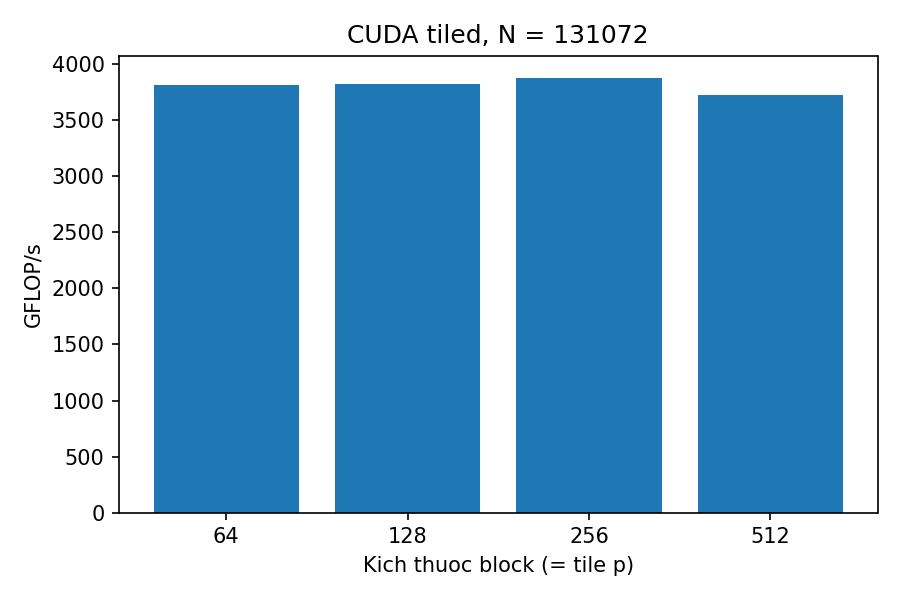
\includegraphics[width=0.8\linewidth]{block_size}
\caption{Hiệu năng kernel tiled theo kích thước khối ($N=131072$).}
\label{fig:block_size}
\end{figure}

$B=256$ cho kết quả tốt nhất, nhưng bốn cấu hình chỉ chênh nhau dưới 4\% (Bảng~\ref{tab:block-size}). Khối nhỏ (64, 128) tái sử dụng mỗi tile ít lần hơn; khối lớn (512) dùng nhiều tài nguyên hơn trên mỗi SM, giảm số khối chạy đồng thời (occupancy). Lựa chọn kích thước khối là cân bằng giữa hai yếu tố này; $B=256$ phù hợp trong phạm vi thí nghiệm, không phải giá trị tối ưu cho mọi GPU.

\subsubsection{Chi phí truyền dữ liệu}

\begin{table}[H]
\centering\small
\begin{tabular}{rrrrrr}
\toprule
\textbf{$N$} & \textbf{H2D (ms)} & \textbf{D2H (ms)} & \textbf{Kernel (ms)} & \textbf{Tỷ lệ truyền} & \textbf{GFLOP/s} \\
\midrule
4096 & 0.090 & 0.066 & 2.569 & 5.72\% & 1306.18 \\
16384 & 0.288 & 0.178 & 15.663 & 2.89\% & 3427.62 \\
65536 & 0.780 & 0.684 & 212.138 & 0.69\% & 4049.23 \\
131072 & 1.230 & 1.231 & 839.962 & 0.29\% & 4090.63 \\
\bottomrule
\end{tabular}
\caption{Chi phí sao chép H2D/D2H so với thời gian tính của kernel tiled (10 bước, $B=256$, một lần đo).}
\label{tab:h2d}
\end{table}

Tỷ lệ thời gian truyền trong tổng thời gian giảm từ 5.72\% ($N=4096$) xuống 0.29\% ($N=131072$), vì lượng dữ liệu truyền tăng theo $O(N)$ còn khối lượng tính tăng theo $O(N^2)$ (Bảng~\ref{tab:h2d}). Kết quả này phù hợp với phân tích theo định luật Gustafson ở Mục~\ref{sec:do-do}: phần không song song hóa được co lại khi bài toán lớn lên. Điều kiện để đạt được tỷ lệ thấp này là dữ liệu được giữ trên GPU suốt mô phỏng; nếu sao chép qua lại ở mỗi bước, chi phí PCIe sẽ đáng kể. Lần đo này là một lần chạy riêng 10 bước, chỉ dùng để đánh giá tỷ lệ sao chép, không thay cho số liệu 5 bước ở Bảng~\ref{tab:naive-tiled}.

\subsection{Nhận xét về phiên bản CUDA}

\begin{itemize}
\item \textbf{Đối chiếu với lý thuyết hiệu năng.} Kernel tiled đạt cao nhất 4675.87 GFLOP/s ($N=16384$), khoảng 57.7\% đỉnh FP32 lý thuyết 8100 GFLOP/s của T4; ở $N \ge 65536$, hiệu năng khoảng 3880--4090 GFLOP/s (48--51\% đỉnh). Theo mô hình roofline \eqref{eq:roofline}, kernel tiled với $B=256$ có cường độ tính toán vượt xa điểm cân bằng, tức là bị giới hạn bởi tính toán chứ không bởi bộ nhớ.
\item \textbf{Khoảng cách tới đỉnh lý thuyết} đến từ: hàm \code{rsqrtf()} chạy trên đơn vị SFU có thông lượng thấp hơn FP32 thường; chi phí hai lệnh \code{\_\_syncthreads()} mỗi tile; chi phí điều khiển vòng lặp; occupancy bị giới hạn bởi thanh ghi và shared memory; vòng trong mới chỉ mở 8 lần (\code{\#pragma unroll 8}) và mỗi luồng mới tính một vật thể, chưa thử cho mỗi luồng tính nhiều vật thể (thread coarsening). Ở $N$ rất lớn, T4 (giới hạn 70 W) có thể hạ xung khi kernel chạy liên tục hàng trăm mili giây.
\item \textbf{So với GPU Gems 3.} Tài liệu gốc báo cáo khoảng 250 GFLOP/s trên GeForce 8800 GTX~\cite{gpugems3}; kết quả trên T4 cao hơn khoảng 18.7 lần, chủ yếu nhờ phần cứng mới hơn với nhiều nhân CUDA hơn.
\end{itemize}

\section{So sánh tổng hợp CPU và GPU}
\label{sec:tong-hop}

\subsection{Kết quả tổng hợp}

Bảng~\ref{tab:tong-hop} tổng hợp thời gian mỗi bước của bốn phiên bản trong cùng một lần đo (môi trường ở Bảng~\ref{tab:moi-truong}); Hình~\ref{fig:time_vs_n} vẽ các số liệu này trên thang log--log.

\begin{table}[H]
\centering\small
\setlength{\tabcolsep}{3pt}
\begin{tabular}{rrrrrrrr}
\toprule
\textbf{$N$} & \textbf{Tuần tự} & \textbf{OpenMP 16} & \textbf{OpenMP/} & \textbf{CUDA naive} & \textbf{CUDA tiled} & \textbf{Tiled/} & \textbf{Tiled/} \\
 & \textbf{(ms)} & \textbf{luồng (ms)} & \textbf{tuần tự} & \textbf{(ms)} & \textbf{(ms)} & \textbf{tuần tự} & \textbf{OpenMP} \\
\midrule
1024 & 0.611 & 0.383 & 1.6× & 0.063 & 0.041 & 14.9× & 9.3× \\
2048 & 2.464 & 1.171 & 2.1× & 0.125 & 0.078 & 31.5× & 15.0× \\
4096 & 10.006 & 2.844 & 3.5× & 0.255 & 0.150 & 66.6× & 18.9× \\
8192 & 39.446 & 9.065 & 4.4× & 0.498 & 0.298 & 132.3× & 30.4× \\
16384 & 158.032 & 40.023 & 3.9× & 1.443 & 1.148 & 137.6× & 34.9× \\
32768 & 693.889 & 146.524 & 4.7× & 5.737 & 4.891 & 141.9× & 30.0× \\
65536 & 2742.200 & 629.848 & 4.4× & 26.209 & 21.873 & 125.4× & 28.8× \\
131072 & 11693.782 & 2431.867 & 4.8× & 103.057 & 88.551 & 132.1× & 27.5× \\
\bottomrule
\end{tabular}
\caption{Thời gian mỗi bước và speedup của bốn phiên bản. CPU: $N \le 16384$ đo 5 bước, $N \ge 32768$ đo 1 bước; GPU: 5 bước, $B=256$; mỗi cấu hình lấy lần nhanh nhất trong 3 lần (nguồn: \code{results/summary.md}).}
\label{tab:tong-hop}
\end{table}

\begin{table}[H]
\centering\small
\begin{tabular}{lrr}
\toprule
\textbf{Phiên bản ($N=16384$)} & \textbf{GFLOP/s} & \textbf{So với tuần tự} \\
\midrule
Tuần tự & 34 & 1× \\
OpenMP 16 luồng & 134 & 3.9× \\
CUDA naive & 3721 & 110× \\
CUDA tiled & 4676 & 138× \\
\bottomrule
\end{tabular}
\caption{Hiệu năng của bốn phiên bản ở $N=16384$ (quy ước 20 FLOP/tương tác).}
\label{tab:gflops}
\end{table}

\begin{figure}[H]
\centering
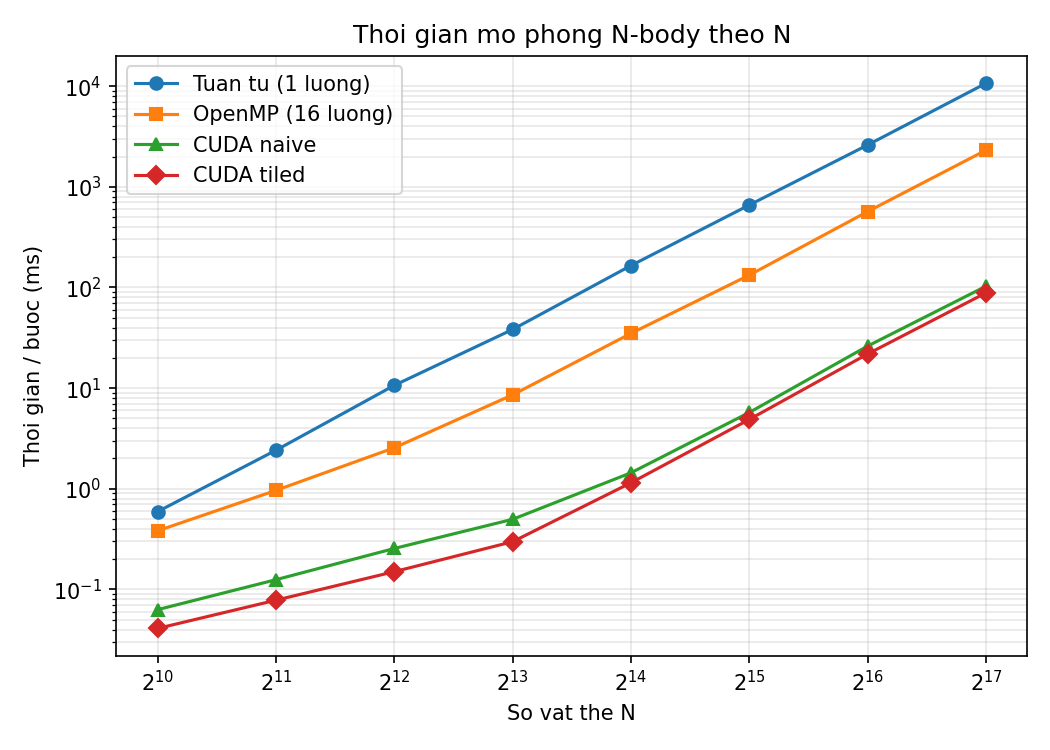
\includegraphics[width=0.85\linewidth]{time_vs_n}
\caption{Thời gian mỗi bước theo $N$ của bốn phiên bản (thang log--log).}
\label{fig:time_vs_n}
\end{figure}

\subsection{Nhận xét}

\textbf{Độ phức tạp $O(N^2)$.} Trên Hình~\ref{fig:time_vs_n}, mỗi lần $N$ tăng gấp đôi thì thời gian tuần tự tăng khoảng 4 lần (ví dụ $39.4 \to 158.0 \to 693.9$ ms), tức độ dốc khoảng 2, đúng với độ phức tạp $O(N^2)$. Các đường OpenMP và CUDA cũng có độ dốc khoảng 2 khi $N$ đủ lớn: song song hóa chỉ dịch đường thẳng xuống dưới, không thay đổi bậc của bài toán.

\textbf{OpenMP.} Với 16 luồng trên i5-12500H, OpenMP nhanh hơn tuần tự 4.4--4.8 lần khi $N \ge 8192$; thí nghiệm riêng trên i7-13620H đạt tối đa 5.91 lần (Mục~\ref{sec:cai-dat-openmp}). Cả hai đều thấp hơn nhiều so với 16 lần lý tưởng vì CPU lai chỉ có 4--6 lõi P, các lõi E chậm hơn và xung nhịp giảm khi nhiều lõi cùng chạy. Với $N$ nhỏ (1024--2048), chi phí tạo và đồng bộ luồng chiếm tỷ lệ lớn nên speedup chỉ 1.6--2.1 lần.

\textbf{GPU so với CPU.} CUDA tiled nhanh hơn bản tuần tự 125--142 lần và nhanh hơn OpenMP 16 luồng 28--35 lần khi $N \ge 8192$. Với $N$ nhỏ, lợi thế giảm còn 15 lần ($N=1024$): lưới chỉ có 4 khối 256 luồng, không đủ lấp đầy 40 SM của T4. Đây là lý do đường CUDA trên Hình~\ref{fig:time_vs_n} thoải hơn (độ dốc nhỏ hơn 2) ở vùng $N \le 8192$. Điều này phù hợp với định luật Gustafson: GPU chỉ phát huy hết khi bài toán đủ lớn.

\textbf{Lưu ý về phép so sánh.} CPU và GPU được đo trên hai máy khác nhau (laptop và Google Colab); CPU dùng \code{-ffast-math}, GPU dùng \code{-use\_fast\_math} (hàm \code{rsqrtf}). Vì vậy các tỷ số CPU--GPU phản ánh bậc độ lớn, không phải phép so sánh trên cùng một hệ thống.

\chapter*{Kết luận}
\addcontentsline{toc}{chapter}{Kết luận}
\label{chap:ket-luan}

\section*{Kết quả đạt được}

Đề tài đã cài đặt bài toán N-body all-pairs theo bốn phiên bản có cùng đầu vào: tuần tự, OpenMP, CUDA naive và CUDA tiled, và đánh giá chúng dựa trên cơ sở lý thuyết tính toán song song ở Chương~\ref{chap:ly-thuyet}. Các kết quả chính:
\begin{itemize}
\item \textbf{Tính đúng đắn:} bản OpenMP khớp bản tuần tự từng bit, hai kernel CUDA khớp với sai số làm tròn khoảng $10^{-8}$; năng lượng toàn phần được bảo toàn tốt ($|\Delta E/E_0| \approx 2.7\times10^{-6}$ sau 2000 bước với $\Delta t=0.002$, $\varepsilon=0.01$).
\item \textbf{CPU đa lõi:} trên i5-12500H (4 lõi P + 8 lõi E), với $N \ge 8192$ OpenMP 16 luồng tăng tốc 4.5--5.0 lần so với tuần tự, đạt khoảng 150--174 GFLOP/s. Vector hóa SIMD đóng góp 1.7--2.9 lần; \code{schedule(dynamic)} nhanh hơn \code{static} 6--24\%, khoảng cách tăng theo $N$, nhờ cân bằng tải giữa lõi P và lõi E.
\item \textbf{GPU:} trên Tesla T4, kernel tiled nhanh hơn bản tuần tự khoảng 121 lần và nhanh hơn OpenMP 16 luồng khoảng 26 lần ở $N=131072$ (cao nhất 144 lần so với tuần tự ở $N=16384$), đạt cao nhất 4.7 TFLOP/s (khoảng 58\% đỉnh lý thuyết). Tiling bằng shared memory nhanh hơn kernel naive 1.16--1.70 lần.
\end{itemize}

\section*{Bài học rút ra}

\begin{itemize}
\item Bài toán có cường độ tính toán cao và các phép tính độc lập như N-body rất phù hợp với GPU; speedup tăng theo kích thước bài toán đúng như định luật Gustafson dự đoán.
\item Speedup thực tế bị giới hạn chủ yếu bởi phần cứng (lõi không đồng nhất, xung nhịp, băng thông bộ nhớ) chứ không phải phần tuần tự của chương trình; định luật Amdahl chỉ là giới hạn trên lý tưởng.
\item Cách truy cập bộ nhớ quan trọng không kém số phép tính: biến thể định luật 3 Newton giảm một nửa phép tính nhưng ở mọi cấu hình lại chậm hơn 1.15--2.3 lần, vì mỗi cặp phải đọc--ghi mảng đệm riêng của luồng và cuối mỗi bước phải cộng dồn các mảng đệm; kernel tiled nhanh hơn naive dù số phép tính như nhau.
\end{itemize}

\section*{Hướng phát triển}

\begin{itemize}
\item \textbf{Thuật toán Barnes--Hut} (cây octree, $O(N\log N)$) hoặc \textbf{Fast Multipole Method} ($O(N)$) để mô phỏng hàng triệu vật thể.
\item \textbf{Nhiều GPU, nhiều máy} bằng MPI: chia các vật thể cho từng tiến trình, trao đổi vị trí mỗi bước theo mô hình vòng (ring).
\item \textbf{Tối ưu kernel CUDA:} thử các mức mở vòng lặp khác (hiện dùng \code{\#pragma unroll 8}), mỗi luồng tính nhiều vật thể (thread coarsening), khai thác định luật 3 Newton theo khối để vẫn giữ được vector hóa.
\item \textbf{Tích phân bậc cao hơn} (leapfrog, Hermite bậc 4) và bước thời gian thích nghi để giảm sai số năng lượng.
\item \textbf{So sánh CPU--GPU trên cùng một máy:} chạy bản CUDA trên GPU RTX 3050 Laptop của chính laptop đã dùng đo CPU, để có tỷ số CPU--GPU không phụ thuộc vào việc dùng hai máy khác nhau.
\item \textbf{Kết hợp CPU và GPU:} chồng lấp truyền dữ liệu với tính toán bằng CUDA streams, chia việc đồng thời cho CPU và GPU.
\end{itemize}


% ---------------- Tai lieu tham khao ----------------
\begin{thebibliography}{99}
\addcontentsline{toc}{chapter}{Tài liệu tham khảo}
\bibitem{gpugems3} L. Nyland, M. Harris, J. Prins, ``Fast N-Body Simulation with CUDA,'' trong H. Nguyen (chủ biên), \emph{GPU Gems 3}, Chương 31, Addison-Wesley, 2007. \url{https://developer.nvidia.com/gpugems/gpugems3/part-v-physics-simulation/chapter-31-fast-n-body-simulation-cuda}
\bibitem{openmp52} OpenMP Architecture Review Board, \emph{OpenMP Application Programming Interface}, phiên bản 5.2, 2021. \url{https://www.openmp.org/specifications/}
\end{thebibliography}

\end{document}
